\begin{center}
\underline{\Large{T.P.Integrador: Edificio N°3}}
\end{center}

A partir de la planta estructural y los datos entregados, proceder al dimensionado de los siguientes
componentes un edificio de hormigón armado según las indicaciones entregadas en el Programa de
Clases Prácticas.\\
\textbf{Grupo 3}\\
El destino del edificio es el de una asociación de jubilados en la ciudad de Trelew.\\
Condición de exposición según CIRSOC 201-05: A2\\
Hormigón H-25 (s/ CIRSOC 201-05) - Hormigón H-21 (s/ CIRSOC 201-82) - Acero ADN 42/50.\\
Características de la estructura:\\
\begin{enumerate}
\item A continuación se anexa la tabla de usos de cada una de las losas de la estructura.
\begin{figure}[H]
\begin{center}
     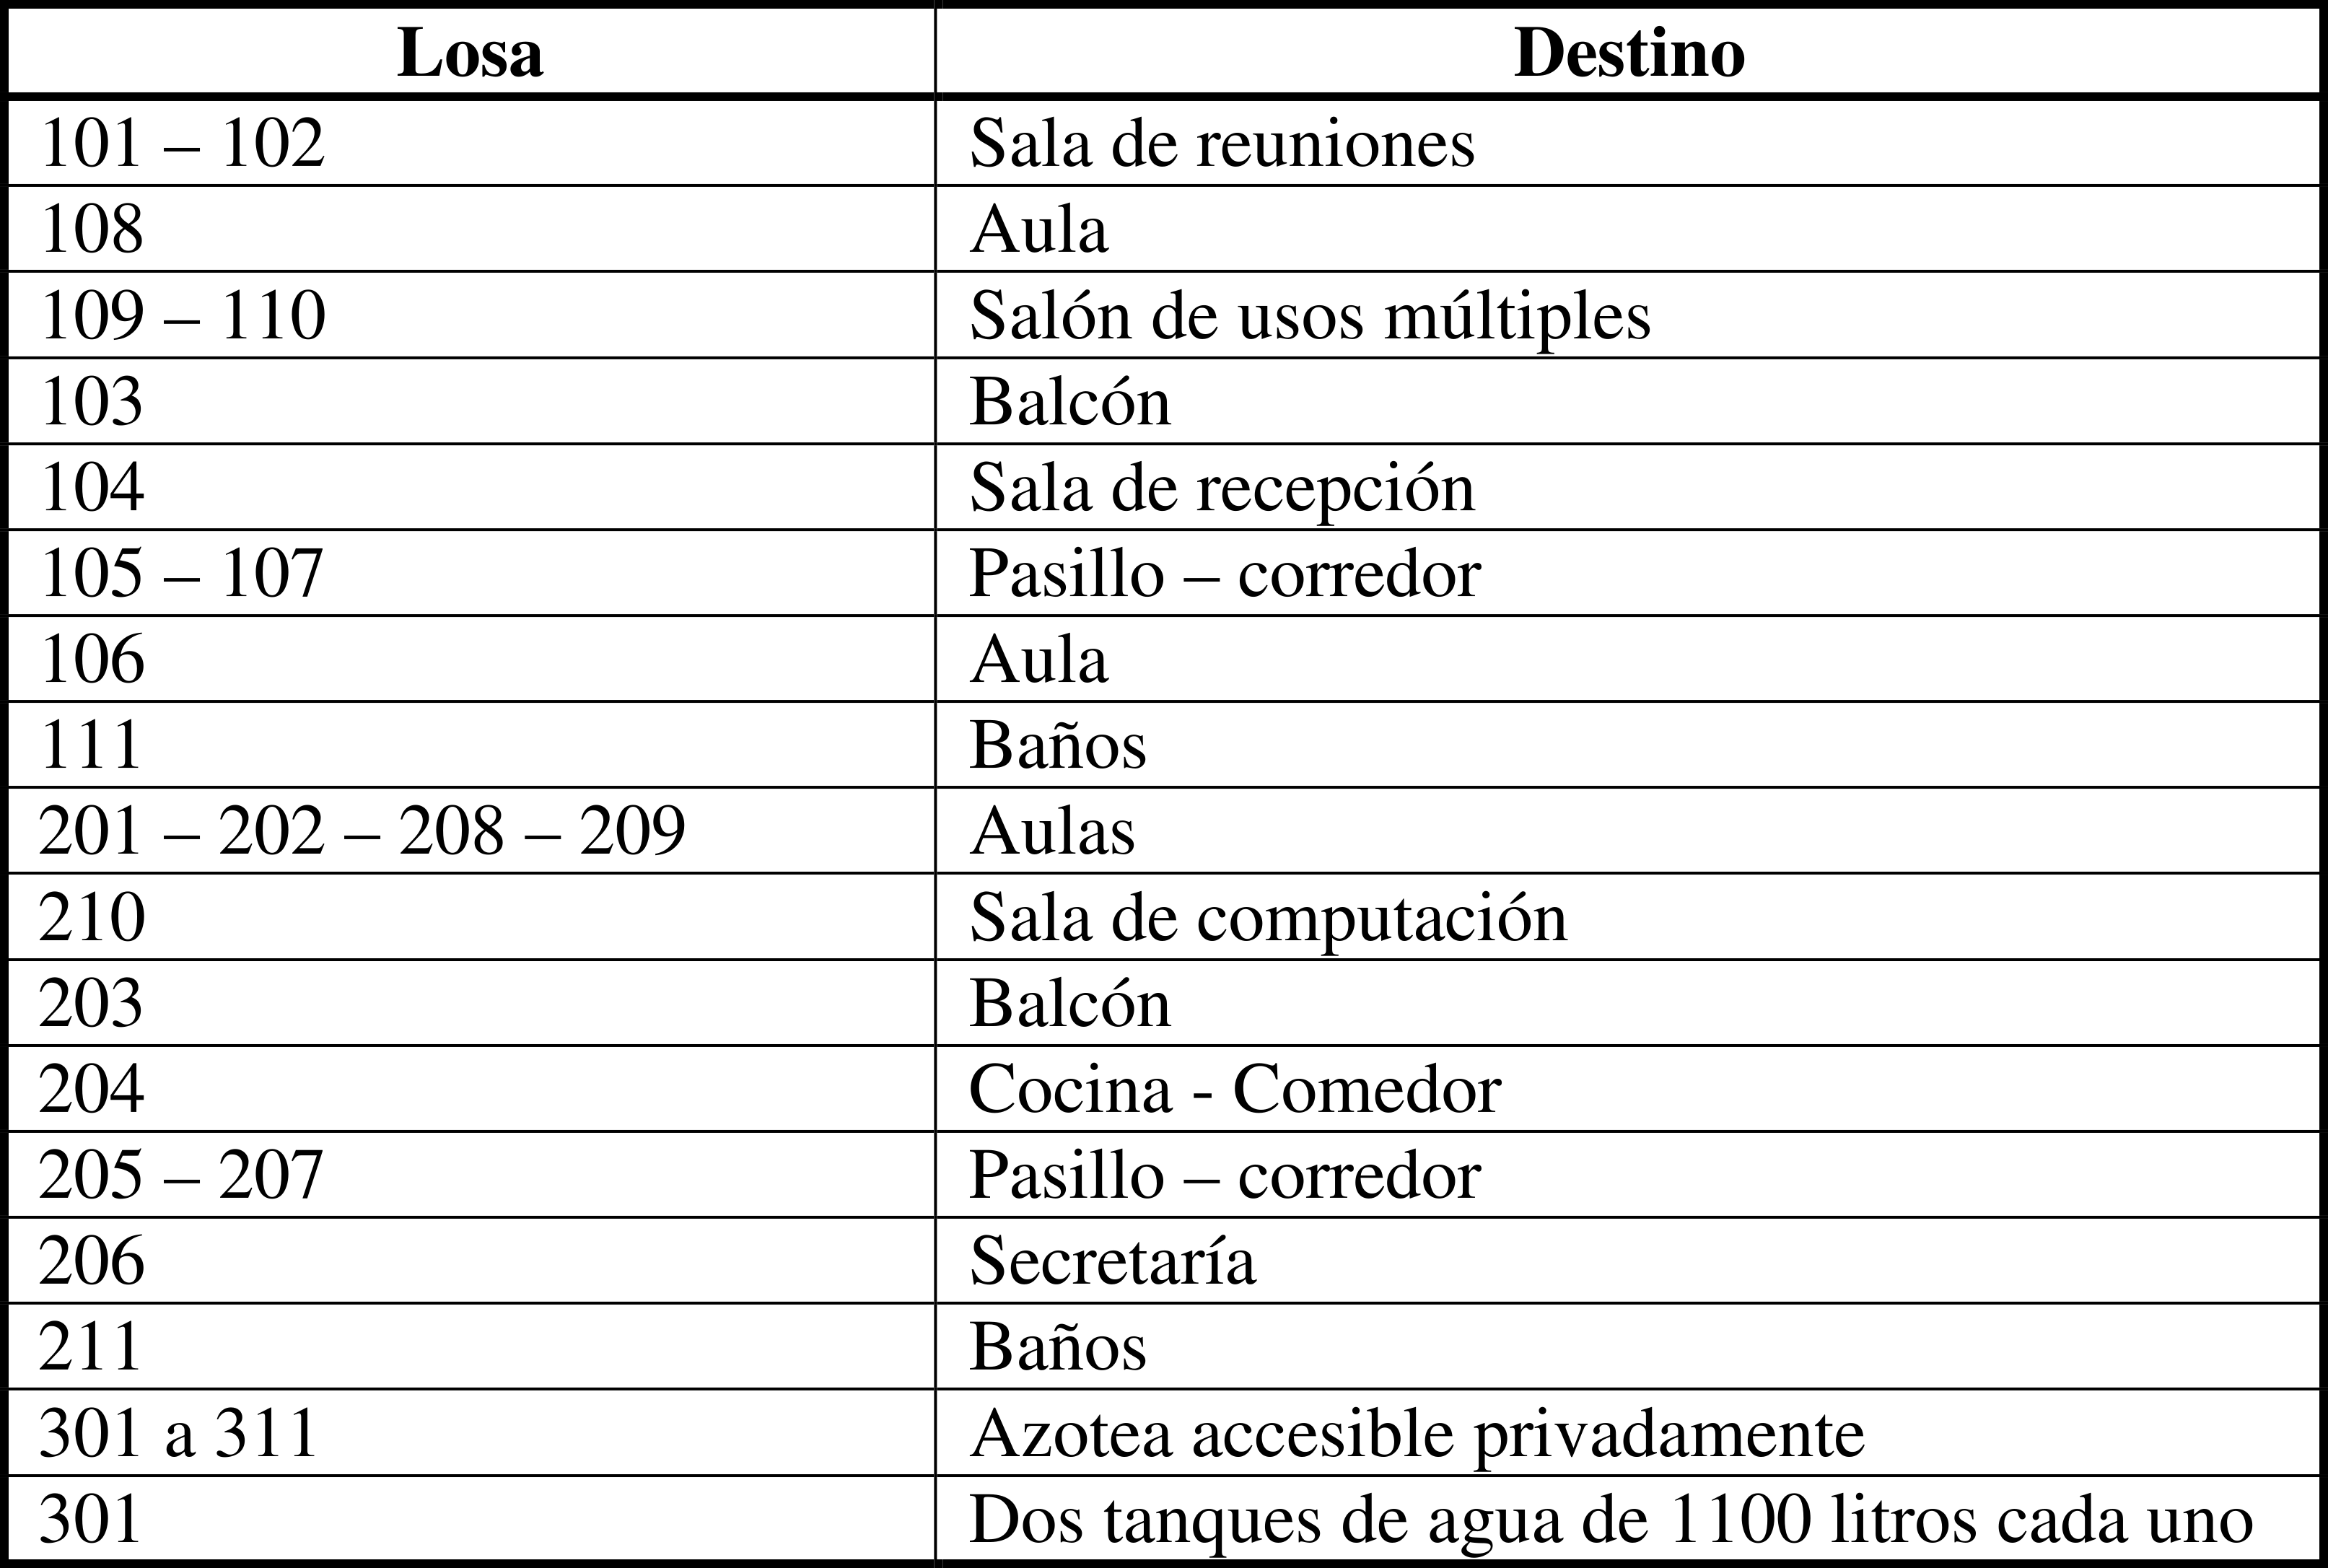
\includegraphics[scale = 0.8]{chapters/chapter_1/images/tabla_de_usos.png}
\end{center}
\end{figure}
\item Los apeos de mampostería en losas se han indicado en la planta con líneas de trazo. Todas las vigas
interiores y exteriores soportan muros de mampostería de 0,20 m de espesor de ladrillo común con
excepción de las vigas 126, 127, 226 y 227. La azotea posee un murete perimetral de 1 m de altura de
0,20 m de espesor de ladrillo común.
\item Considerar para las losas de azotea, la carga generada por el respectivo contrapiso con pendientes
equivalentes al 2\% para desagües pluviales. Las azoteas son accesibles.
\item Las alturas de los niveles resultan de 3,50 m para la planta baja, y de 3 m para los restantes niveles.
\item Los paquetes estructurales de las losas corresponden a los siguientes esquemas:
\begin{figure}[H]
\begin{center}
     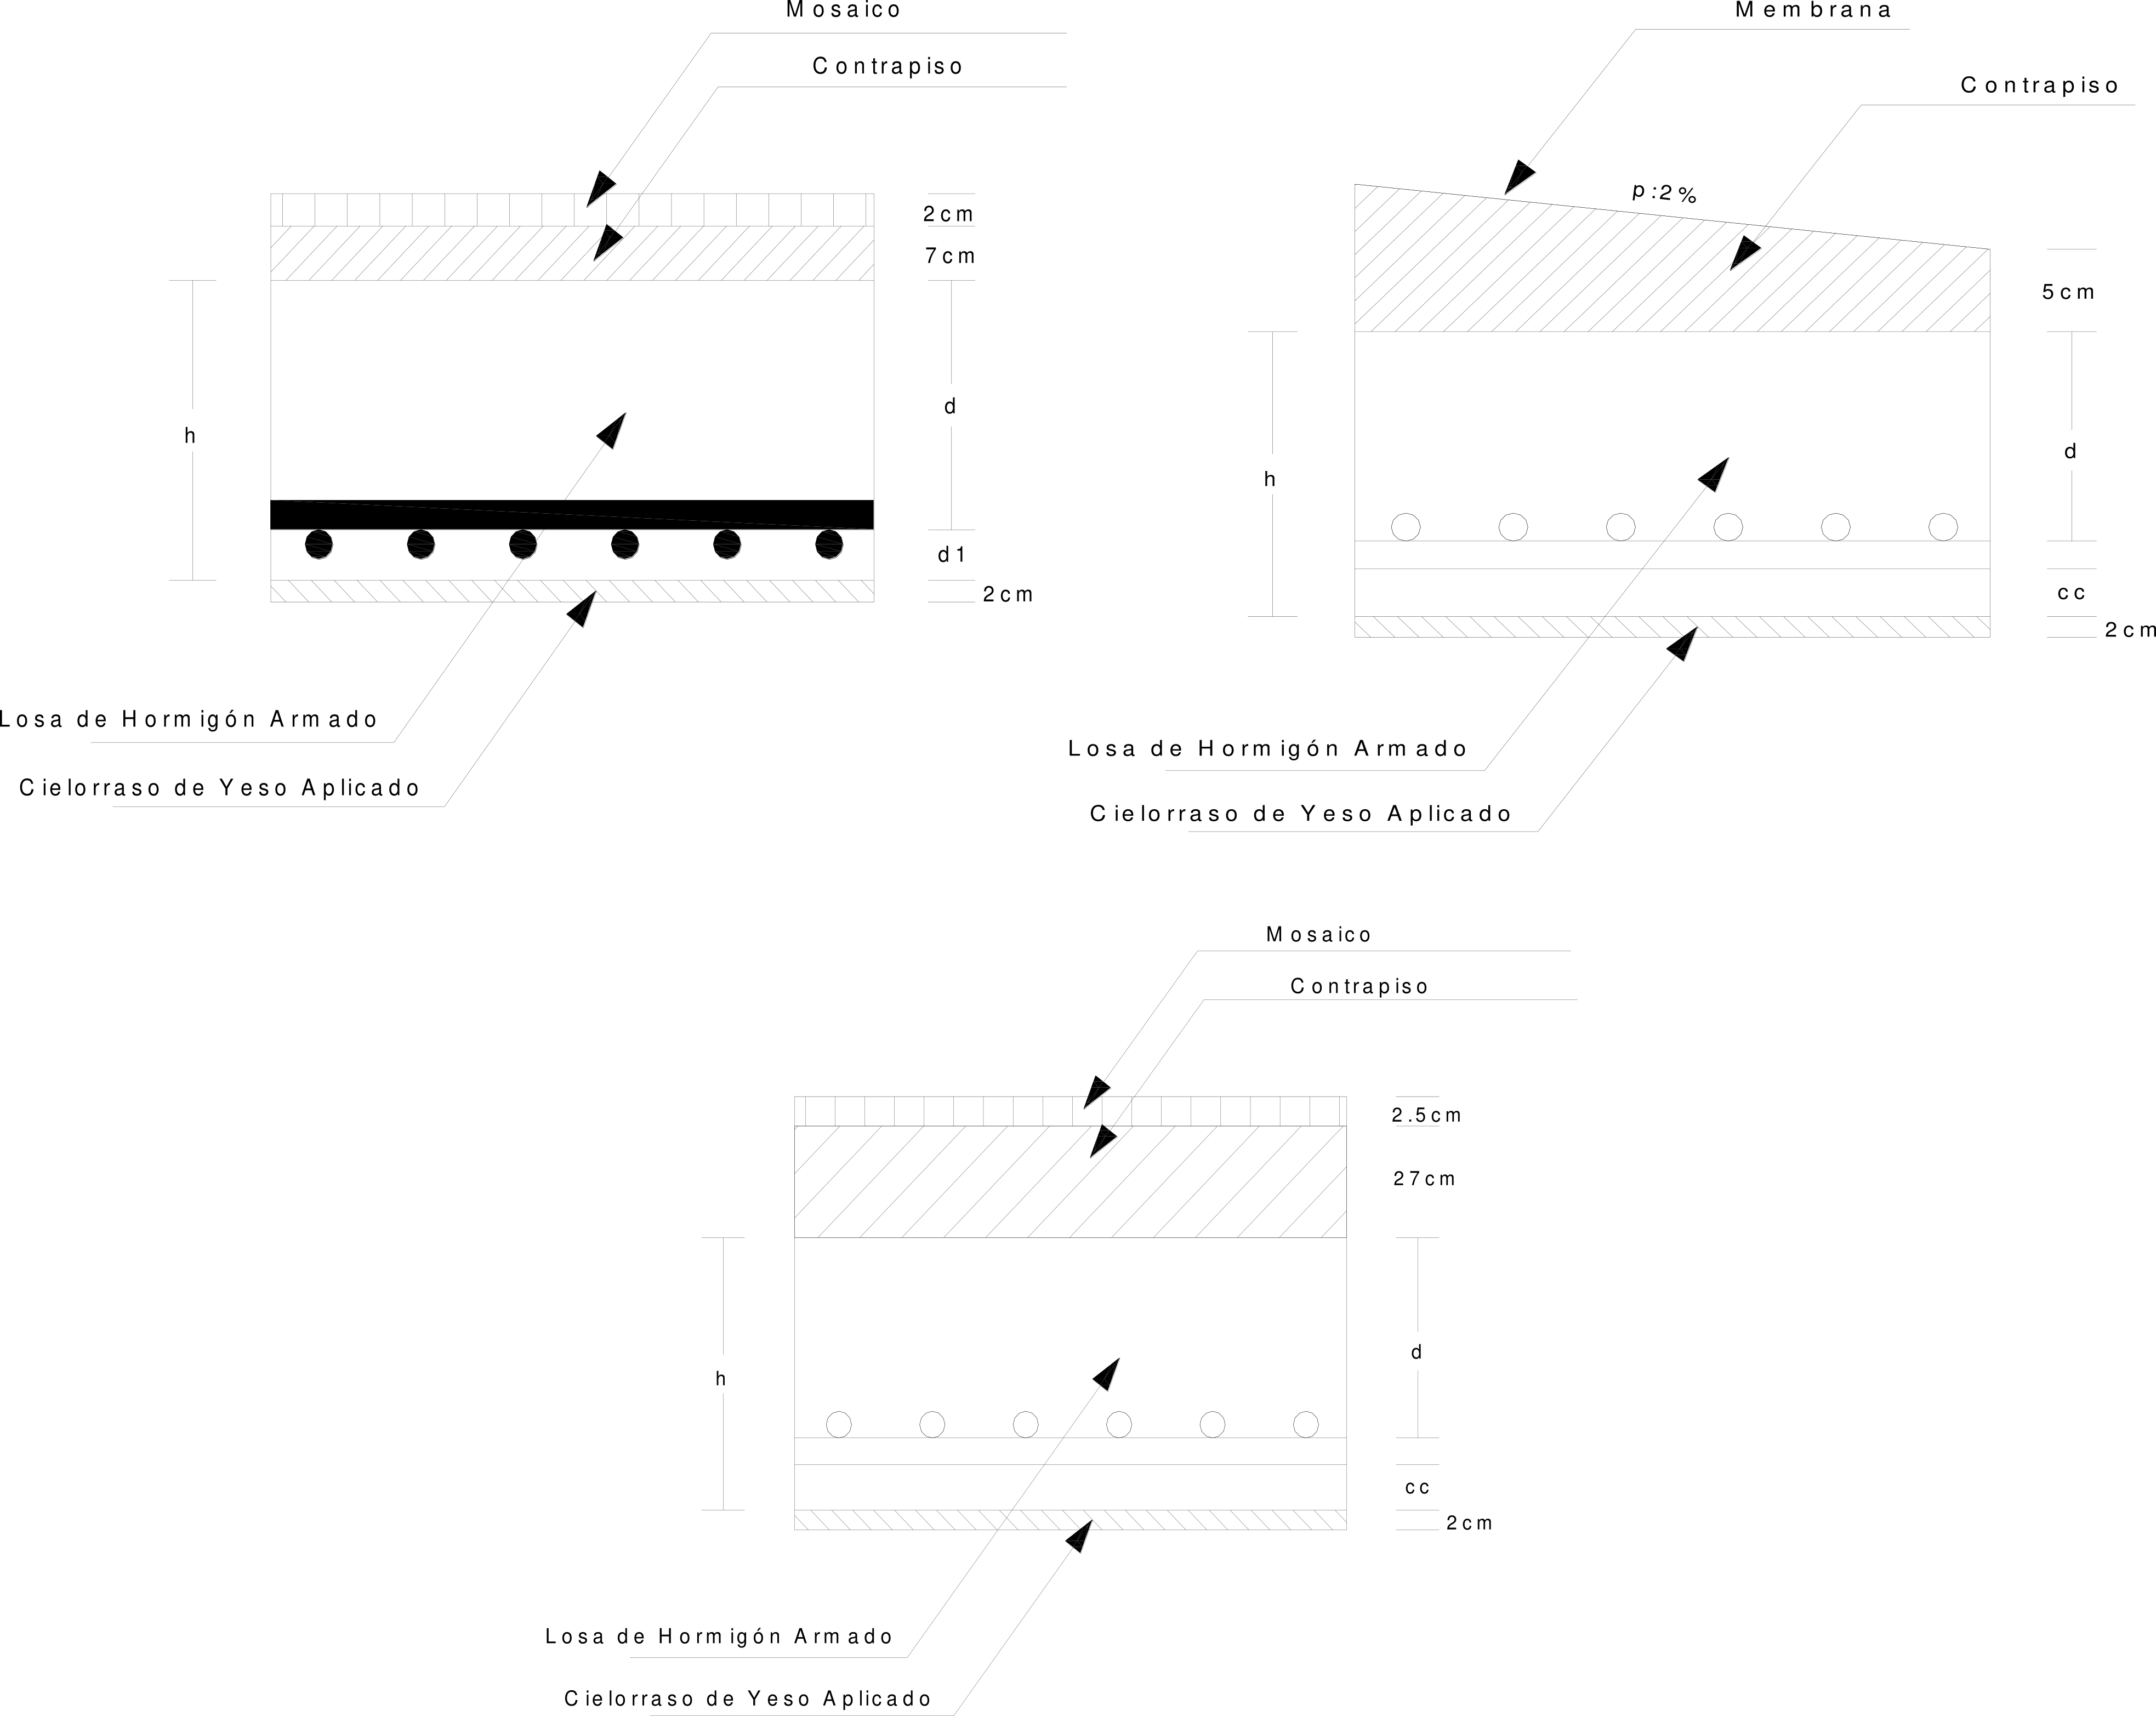
\includegraphics[scale = 0.8]{chapters/chapter_1/images/paquetes.png}
\end{center}
\end{figure}
\item Los suelos sobre los que se funda la estructura poseen una tensión admisible del suelo de 2,5 kg/cm²,
y no resultan agresivos. El nivel de fundación es de -1,5 m.
\end{enumerate}

\newpage
\begin{center}
\underline{Cálculo de Losas}
\end{center}
\underline{Datos:}\\
Hormigón H-25 $\Rightarrow f'c = 250 \frac{Kg}{cm^2} = 25 MPa$\\
Acero ADN 42/50 $\Rightarrow fy = 4200 \frac{Kg}{cm^2} = 420 MPa$\\
Recubrimiento Cc = 2cm\\

\begin{enumerate}
\item \underline{Predimensionado de losas en dos direcciones. L208}

Losa L208.
\begin{align*}
& l_x = 3.90m \\
& l_y = 5.20m \\
& h_{losa} = 14cm\\
\end{align*}

Vigas.
\begin{align*}
& b_w = 20cm \qquad b_w = 20cm\\
& h = 40cm \qquad h = 40cm
\end{align*}

Momento de inercia de la viga.
\begin{align*}
& I_{B} = \frac{b \cdot h^3}{12} = \frac{20cm \cdot (40cm)^3}{12} = \framebox{$106667cm^4$}
\end{align*}

Momento de inercia de la losa.
\begin{align*}
& I_{sy} = \frac{b \cdot h^3}{12} = \frac{520cm \cdot (14cm)^3}{12} = \framebox{$118907cm^4$}\\
& I_{sx} = \frac{b \cdot h^3}{12} = \frac{390cm \cdot (14cm)^3}{12} = \framebox{$89180cm^4$}\\
& \alpha_y = \frac{I_B}{I_{sy}} = \frac{106667cm^4}{118907cm^4} = \framebox{$0.90$} \\
& \alpha_x = \frac{I_B}{I_{sx}} = \frac{106667cm^4}{89180cm^4} = \framebox{$1.20$}\\
& \alpha_m = \frac{\alpha_x+\alpha_y}{2} = \frac{(0.90+1.20)}{2} = \framebox{$1.05$}
\end{align*}

\newpage
Dado que $\alpha_m < 2 $ entonces:
\begin{align*}
& \alpha_m = 1.05 < 2 \\
& h \geq = \frac{l_w \cdot (0.80+ \frac{fy}{1400})}{36+ 5 \cdot \beta \cdot (\alpha_m - 0.2)} \\
& h \geq = \frac{520cm \cdot (0.80+ \frac{420MPa}{1400})}{36+ 5 \cdot \frac{520cm}{390cm} \cdot (1.05 - 0.2)} \\
& h \geq \framebox{$13.73cm$} \\
& h_{min} \geq 12cm
\end{align*}

Adopto $\framebox{$h = 14cm$}$ \\
$h_{adoptado} = 14 cm \geq 13.73cm$ Verifica \\

\item \underline{Predimensionado de losas en una dirección}\\

\begin{itemize}
\item Losa L102
\begin{align*}
& h_{min losa} = \frac{ln}{24} = \frac{250cm}{24} = \framebox{$10.41cm$} \quad \text{De tabla 9.5.a}
\end{align*}
$h_{adoptado} = \framebox{$14 cm$} \geq 10.41cm$ Verifica \\
\item Losa L103
\begin{align*}
& h_{min losa} = \frac{ln}{10} = \frac{130cm}{10} = \framebox{$13cm$} \quad \text{De tabla 9.5.a}
\end{align*}
$h_{adoptado} = \framebox{$14 cm$} \geq 13cm$ Verifica \\
\end{itemize}

\item \underline{Análisis de cargas}\\

\begin{itemize}
\item Losa L101 y L102: Sala de Reuniones
\begin{align*}
& \text{Peso propio} \rightarrow 0.14m \cdot 2500 \frac{Kg}{m^3} = 350 \frac{Kg}{m^2}\\
& \text{Contrapiso} \rightarrow 0.07m \cdot 1600 \frac{Kg}{m^3} = 112 \frac{Kg}{m^2}\\
& \text{Piso + Carpeta} \rightarrow 0.02m \cdot 2000 \frac{Kg}{m^3} = 40 \frac{Kg}{m^2}\\
& \text{Cielorraso aplicado} \rightarrow  0.02m \cdot 1300 \frac{Kg}{m^3} = 26 \frac{Kg}{m^2}\\
& D = 528 \frac{Kg}{m^2}\\
& L = 500 \frac{Kg}{m^2} \rightarrow \text{Según CIRSOC 101-05 - Capítulo 4}\\
& q_u = 1.2 \cdot D + 1.6 \cdot L = 1.2 \cdot 528 \frac{Kg}{m^2} + 1.6 \cdot 500 \frac{Kg}{m^2} = 1433.6 \frac{Kg}{m^2} \Rightarrow \framebox{$1.43 \frac{t}{m^2}$} \\
& q_u = 1.4 \cdot D = 1.4 \cdot 528 \frac{Kg}{m^2} = 739.2 \frac{Kg}{m^2} \Rightarrow 0.739 \frac{t}{m^2}
\end{align*}

\item Losa L103 y L203: Balcón
\begin{align*}
& \text{Peso propio} \rightarrow 0.14m \cdot 2500 \frac{Kg}{m^3} = 350 \frac{Kg}{m^2}\\
& \text{Contrapiso} \rightarrow 0.07m \cdot 1600 \frac{Kg}{m^3} = 112 \frac{Kg}{m^2}\\
& \text{Piso + Carpeta} \rightarrow 0.02m \cdot 2000 \frac{Kg}{m^3} = 40 \frac{Kg}{m^2}\\
& \text{Cielorraso aplicado} \rightarrow  0.02m \cdot 1300 \frac{Kg}{m^3} = 26 \frac{Kg}{m^2}\\
& D = 528 \frac{Kg}{m^2}\\
& L = 500 \frac{Kg}{m^2} \rightarrow \text{Según CIRSOC 101-05 - Capítulo 4}\\
& q_u = 1.2 \cdot D + 1.6 \cdot L = 1.2 \cdot 528 \frac{Kg}{m^2} + 1.6 \cdot 500 \frac{Kg}{m^2} = 1433.6 \frac{Kg}{m^2} \Rightarrow \framebox{$1.43 \frac{t}{m^2}$} \\
& q_u = 1.4 \cdot D = 1.4 \cdot 528 \frac{Kg}{m^2} = 739.2 \frac{Kg}{m^2} \Rightarrow 0.739 \frac{t}{m^2}
\end{align*}

\item Losa L111 : Baños
\begin{align*}
& \text{Peso propio} \rightarrow 0.14m \cdot 2500 \frac{Kg}{m^3} = 350 \frac{Kg}{m^2}\\
& \text{Contrapiso} \rightarrow 0.27m \cdot 1600 \frac{Kg}{m^3} = 432 \frac{Kg}{m^2}\\
& \text{Piso + Carpeta} \rightarrow 0.025m \cdot 2000 \frac{Kg}{m^3} = 50 \frac{Kg}{m^2}\\
& \text{Cielorraso aplicado} \rightarrow  0.02m \cdot 1300 \frac{Kg}{m^3} = 26 \frac{Kg}{m^2}\\
& D = 858 \frac{Kg}{m^2}\\
& L = 300 \frac{Kg}{m^2} \rightarrow \text{Según CIRSOC 101-05 - Capítulo 4}\\
& q_u = 1.2 \cdot D + 1.6 \cdot L = 1.2 \cdot 858 \frac{Kg}{m^2} + 1.6 \cdot 300 \frac{Kg}{m^2} = 1509.6 \frac{Kg}{m^2} \Rightarrow \framebox{$1.50 \frac{t}{m^2}$}\\
& q_u = 1.4 \cdot D = 1.4 \cdot 858 \frac{Kg}{m^2} = 1201.2 \frac{Kg}{m^2} \Rightarrow 1.20 \frac{t}{m^2}
\end{align*}

\item Losa L211: Baños
\begin{align*}
& \text{Peso propio} \rightarrow 0.14m \cdot 2500 \frac{Kg}{m^3} = 350 \frac{Kg}{m^2}\\
& \text{Contrapiso} \rightarrow 0.27m \cdot 1600 \frac{Kg}{m^3} = 432 \frac{Kg}{m^2}\\
& \text{Piso + Carpeta} \rightarrow 0.025m \cdot 2000 \frac{Kg}{m^3} = 50 \frac{Kg}{m^2}\\
& \text{Cielorraso aplicado} \rightarrow  0.02m \cdot 1300 \frac{Kg}{m^3} = 26 \frac{Kg}{m^2}\\
& D = 858 \frac{Kg}{m^2}\\
& \frac{l_1}{l_2} = \frac{3.60m}{3.60m} = 1 \Rightarrow \text{De tabla tenemos los coeficientes} \\
& \text{Muro paralelo al lado corto} = 1.60 \\
& \text{Muro paralelo al lado largo} = 1.60 \\
& D_{pared} = \frac{(0.10m \cdot (1m+1m+2.28) \cdot 2.7m \cdot 1700 \frac{Kg}{m^3}) \cdot 1.60}{3.60m \cdot 3.60m}\\
& + \frac{(0.10m \cdot 1.81m \cdot 2.7m \cdot 1700 \frac{Kg}{m^3}) \cdot 1.60}{3.60m \cdot 3.60m}\\
& D_{pared} = 345 \frac{Kg}{m^2} \\
& D_{total} = 858 \frac{Kg}{m^2} + 345 \frac{Kg}{m^2} = 1203 \frac{Kg}{m^2}\\
& L = 300 \frac{Kg}{m^2} \rightarrow \text{Según CIRSOC 101-05 - Capítulo 4}\\
& q_u = 1.2 \cdot D_{total} + 1.6 \cdot L = 1.2 \cdot 1203 \frac{Kg}{m^2} + 1.6 \cdot 300 \frac{Kg}{m^2} = 1923.6 \frac{Kg}{m^2} \Rightarrow \framebox{$1.92 \frac{t}{m^2}$}\\
& q_u = 1.4 \cdot D_{total} = 1.4 \cdot 1203 \frac{Kg}{m^2} = 1684.2 \frac{Kg}{m^2} \Rightarrow 1.68 \frac{t}{m^2}
\end{align*}

\item Losa L104: Recepción
\begin{align*}
& \text{Peso propio} \rightarrow 0.14m \cdot 2500 \frac{Kg}{m^3} = 350 \frac{Kg}{m^2}\\
& \text{Contrapiso} \rightarrow 0.07m \cdot 1600 \frac{Kg}{m^3} = 112 \frac{Kg}{m^2}\\
& \text{Piso + Carpeta} \rightarrow 0.02m \cdot 2000 \frac{Kg}{m^3} = 40 \frac{Kg}{m^2}\\
& \text{Cielorraso aplicado} \rightarrow  0.02m \cdot 1300 \frac{Kg}{m^3} = 26 \frac{Kg}{m^2}\\
& D = 528 \frac{Kg}{m^2}\\
& L = 250 \frac{Kg}{m^2} \rightarrow \text{Según CIRSOC 101-05 - Capítulo 4}\\
& q_u = 1.2 \cdot D + 1.6 \cdot L = 1.2 \cdot 528 \frac{Kg}{m^2} + 1.6 \cdot 250 \frac{Kg}{m^2} = 1033.3 \frac{Kg}{m^2} \Rightarrow \framebox{$1.03 \frac{t}{m^2}$} \\
& q_u = 1.4 \cdot D = 1.4 \cdot 528 \frac{Kg}{m^2} = 739.2 \frac{Kg}{m^2} \Rightarrow 0.739 \frac{t}{m^2}
\end{align*}

\item Losa L105, L107, L205 y L207: Pasillo - Corredor
\begin{align*}
& \text{Peso propio} \rightarrow 0.14m \cdot 2500 \frac{Kg}{m^3} = 350 \frac{Kg}{m^2}\\
& \text{Contrapiso} \rightarrow 0.07m \cdot 1600 \frac{Kg}{m^3} = 112 \frac{Kg}{m^2}\\
& \text{Piso + Carpeta} \rightarrow 0.02m \cdot 2000 \frac{Kg}{m^3} = 40 \frac{Kg}{m^2}\\
& \text{Cielorraso aplicado} \rightarrow  0.02m \cdot 1300 \frac{Kg}{m^3} = 26 \frac{Kg}{m^2}\\
& D = 528 \frac{Kg}{m^2}\\
& L = 400 \frac{Kg}{m^2} \rightarrow \text{Según CIRSOC 101-05 - Capítulo 4}\\
& q_u = 1.2 \cdot D + 1.6 \cdot L = 1.2 \cdot 528 \frac{Kg}{m^2} + 1.6 \cdot 400 \frac{Kg}{m^2} = 1273 \frac{Kg}{m^2} \Rightarrow \framebox{$1.27 \frac{t}{m^2}$} \\
& q_u = 1.4 \cdot D = 1.4 \cdot 528 \frac{Kg}{m^2} = 739.2 \frac{Kg}{m^2} \Rightarrow 0.739 \frac{t}{m^2}
\end{align*}

\item Losa L106, L201, L208 y L209: Aulas
\begin{align*}
& \text{Peso propio} \rightarrow 0.14m \cdot 2500 \frac{Kg}{m^3} = 350 \frac{Kg}{m^2}\\
& \text{Contrapiso} \rightarrow 0.07m \cdot 1600 \frac{Kg}{m^3} = 112 \frac{Kg}{m^2}\\
& \text{Piso + Carpeta} \rightarrow 0.02m \cdot 2000 \frac{Kg}{m^3} = 40 \frac{Kg}{m^2}\\
& \text{Cielorraso aplicado} \rightarrow  0.02m \cdot 1300 \frac{Kg}{m^3} = 26 \frac{Kg}{m^2}\\
& D = 528 \frac{Kg}{m^2}\\
& L = 300 \frac{Kg}{m^2} \rightarrow \text{Según CIRSOC 101-05 - Capítulo 4}\\
& q_u = 1.2 \cdot D + 1.6 \cdot L = 1.2 \cdot 528 \frac{Kg}{m^2} + 1.6 \cdot 300 \frac{Kg}{m^2} = 1113.6 \frac{Kg}{m^2} \Rightarrow \framebox{$1.11 \frac{t}{m^2}$} \\
& q_u = 1.4 \cdot D = 1.4 \cdot 528 \frac{Kg}{m^2} = 739.2 \frac{Kg}{m^2} \Rightarrow 0.739 \frac{t}{m^2}
\end{align*}

\item Losa L108: Aulas
\begin{align*}
& \text{Peso propio} \rightarrow 0.14m \cdot 2500 \frac{Kg}{m^3} = 350 \frac{Kg}{m^2}\\
& \text{Contrapiso} \rightarrow 0.07m \cdot 1600 \frac{Kg}{m^3} = 112 \frac{Kg}{m^2}\\
& \text{Piso + Carpeta} \rightarrow 0.02m \cdot 2000 \frac{Kg}{m^3} = 40 \frac{Kg}{m^2}\\
& \text{Cielorraso aplicado} \rightarrow  0.02m \cdot 1300 \frac{Kg}{m^3} = 26 \frac{Kg}{m^2}\\
& D = 528 \frac{Kg}{m^2}\\
& \frac{l_1}{l_2} = \frac{3.9m}{5.2m} = 0.75 \Rightarrow 0.8 \Rightarrow \text{De tabla tenemos los coeficientes} \\
& \text{Muro paralelo al lado corto} = 1.50 \\
& \text{Muro paralelo al lado largo} = 1.70 \\
& D_{pared} = \frac{2.6m \cdot 2.7m \cdot 0.1m \cdot 1700\frac{Kg}{m^3}}{3.9m \cdot 5.2m} \cdot 1.50 + \frac{2.6m \cdot 2.7m \cdot 0.1m \cdot 1700\frac{Kg}{m^3}}{3.9m \cdot 5.2m} \cdot 1.70 \\
& D_{pared} = 130.6 \frac{Kg}{m^2} \\
& D_{total} = 528 \frac{Kg}{m^2} + 130.6 \frac{Kg}{m^2} = 658.6 \frac{Kg}{m^2}\\
& L = 300 \frac{Kg}{m^2} \rightarrow \text{Según CIRSOC 101-05 - Capítulo 4}\\
& q_u = 1.2 \cdot D_{total} + 1.6 \cdot L = 1.2 \cdot 658.6 \frac{Kg}{m^2} + 1.6 \cdot 300 \frac{Kg}{m^2} = 1270.32 \frac{Kg}{m^2} \Rightarrow \framebox{$1.27 \frac{t}{m^2}$} \\
& q_u = 1.4 \cdot D_{total} = 1.4 \cdot 658.6 \frac{Kg}{m^2} = 922.04 \frac{Kg}{m^2} \Rightarrow 0.92 \frac{t}{m^2}
\end{align*}

\item Losa L202: Aulas
\begin{align*}
& \text{Peso propio} \rightarrow 0.14m \cdot 2500 \frac{Kg}{m^3} = 350 \frac{Kg}{m^2}\\
& \text{Contrapiso} \rightarrow 0.07m \cdot 1600 \frac{Kg}{m^3} = 112 \frac{Kg}{m^2}\\
& \text{Piso + Carpeta} \rightarrow 0.02m \cdot 2000 \frac{Kg}{m^3} = 40 \frac{Kg}{m^2}\\
& \text{Cielorraso aplicado} \rightarrow  0.02m \cdot 1300 \frac{Kg}{m^3} = 26 \frac{Kg}{m^2}\\
& D = 528 \frac{Kg}{m^2}\\
& D_{pared} = 1m \cdot 2.7m \cdot 0.1m \cdot 1700\frac{Kg}{m^3} \\
& D_{pared} = 459 Kg \\
& L = 300 \frac{Kg}{m^2} \rightarrow \text{Según CIRSOC 101-05 - Capítulo 4}\\
& q_u = 1.2 \cdot D + 1.6 \cdot L = 1.2 \cdot 528 \frac{Kg}{m^2} + 1.6 \cdot 300 \frac{Kg}{m^2} = 1113.6 \frac{Kg}{m^2} \Rightarrow \framebox{$1.11 \frac{t}{m^2}$} \\
& q_u = 1.4 \cdot D = 1.4 \cdot 528 \frac{Kg}{m^2} = 739.2 \frac{Kg}{m^2} \Rightarrow 0.739 \frac{t}{m^2} \\
& q_u = 1.2 \cdot D_{pared} = 1.2 \cdot 459 Kg = 550.8 Kg \Rightarrow 0.55 t
\end{align*}

\item Losa L206: Secretaria
\begin{align*}
& \text{Peso propio} \rightarrow 0.14m \cdot 2500 \frac{Kg}{m^3} = 350 \frac{Kg}{m^2}\\
& \text{Contrapiso} \rightarrow 0.07m \cdot 1600 \frac{Kg}{m^3} = 112 \frac{Kg}{m^2}\\
& \text{Piso + Carpeta} \rightarrow 0.02m \cdot 2000 \frac{Kg}{m^3} = 40 \frac{Kg}{m^2}\\
& \text{Cielorraso aplicado} \rightarrow  0.02m \cdot 1300 \frac{Kg}{m^3} = 26 \frac{Kg}{m^2}\\
& D = 528 \frac{Kg}{m^2}\\
& L = 250 \frac{Kg}{m^2} \rightarrow \text{Según CIRSOC 101-05 - Capítulo 4}\\
& q_u = 1.2 \cdot D + 1.6 \cdot L = 1.2 \cdot 528 \frac{Kg}{m^2} + 1.6 \cdot 250 \frac{Kg}{m^2} = 1033.3 \frac{Kg}{m^2} \Rightarrow \framebox{$1.03 \frac{t}{m^2}$} \\
& q_u = 1.4 \cdot D = 1.4 \cdot 528 \frac{Kg}{m^2} = 739.2 \frac{Kg}{m^2} \Rightarrow 0.739 \frac{t}{m^2}
\end{align*}

\item Losa L204: Cocina - Comedor
\begin{align*}
& \text{Peso propio} \rightarrow 0.14m \cdot 2500 \frac{Kg}{m^3} = 350 \frac{Kg}{m^2}\\
& \text{Contrapiso} \rightarrow 0.27m \cdot 1600 \frac{Kg}{m^3} = 432 \frac{Kg}{m^2}\\
& \text{Piso + Carpeta} \rightarrow 0.025m \cdot 2000 \frac{Kg}{m^3} = 50 \frac{Kg}{m^2}\\
& \text{Cielorraso aplicado} \rightarrow  0.02m \cdot 1300 \frac{Kg}{m^3} = 26 \frac{Kg}{m^2}\\
& D = 858 \frac{Kg}{m^2}\\
& L = 500 \frac{Kg}{m^2} \rightarrow \text{Según CIRSOC 101-05 - Capítulo 4}\\
& q_u = 1.2 \cdot D + 1.6 \cdot L = 1.2 \cdot 858 \frac{Kg}{m^2} + 1.6 \cdot 500 \frac{Kg}{m^2} = 1829.6 \frac{Kg}{m^2} \Rightarrow \framebox{$1.82 \frac{t}{m^2}$}\\
& q_u = 1.4 \cdot D = 1.4 \cdot 858 \frac{Kg}{m^2} = 1201.2 \frac{Kg}{m^2} \Rightarrow 1.20 \frac{t}{m^2}
\end{align*}

\item Losa L210: Sala de Computación
\begin{align*}
& \text{Peso propio} \rightarrow 0.14m \cdot 2500 \frac{Kg}{m^3} = 350 \frac{Kg}{m^2}\\
& \text{Contrapiso} \rightarrow 0.07m \cdot 1600 \frac{Kg}{m^3} = 112 \frac{Kg}{m^2}\\
& \text{Piso + Carpeta} \rightarrow 0.02m \cdot 2000 \frac{Kg}{m^3} = 40 \frac{Kg}{m^2}\\
& \text{Cielorraso aplicado} \rightarrow  0.02m \cdot 1300 \frac{Kg}{m^3} = 26 \frac{Kg}{m^2}\\
& D = 528 \frac{Kg}{m^2}\\
& L = 500 \frac{Kg}{m^2} \rightarrow \text{Según CIRSOC 101-05 - Capítulo 4}\\
& q_u = 1.2 \cdot D + 1.6 \cdot L = 1.2 \cdot 528 \frac{Kg}{m^2} + 1.6 \cdot 500 \frac{Kg}{m^2} = 1433.6 \frac{Kg}{m^2} \Rightarrow \framebox{$1.43 \frac{t}{m^2}$} \\
& q_u = 1.4 \cdot D = 1.4 \cdot 528 \frac{Kg}{m^2} = 739.2 \frac{Kg}{m^2} \Rightarrow 0.739 \frac{t}{m^2}
\end{align*}

\item Losa L109: Sala de Usos Múltiples
\begin{align*}
& \text{Peso propio} \rightarrow 0.14m \cdot 2500 \frac{Kg}{m^3} = 350 \frac{Kg}{m^2}\\
& \text{Contrapiso} \rightarrow 0.07m \cdot 1600 \frac{Kg}{m^3} = 112 \frac{Kg}{m^2}\\
& \text{Piso + Carpeta} \rightarrow 0.02m \cdot 2000 \frac{Kg}{m^3} = 40 \frac{Kg}{m^2}\\
& \text{Cielorraso aplicado} \rightarrow  0.02m \cdot 1300 \frac{Kg}{m^3} = 26 \frac{Kg}{m^2}\\
& D = 528 \frac{Kg}{m^2}\\
& L = 500 \frac{Kg}{m^2} \rightarrow \text{Según CIRSOC 101-05 - Capítulo 4}\\
& q_u = 1.2 \cdot D + 1.6 \cdot L = 1.2 \cdot 528 \frac{Kg}{m^2} + 1.6 \cdot 500 \frac{Kg}{m^2} = 1433.6 \frac{Kg}{m^2} \Rightarrow \framebox{$1.43 \frac{t}{m^2}$} \\
& q_u = 1.4 \cdot D = 1.4 \cdot 528 \frac{Kg}{m^2} = 739.2 \frac{Kg}{m^2} \Rightarrow 0.739 \frac{t}{m^2}
\end{align*}

\item Losa L110: Sala de Usos Múltiples
\begin{align*}
& \text{Peso propio} \rightarrow 0.14m \cdot 2500 \frac{Kg}{m^3} = 350 \frac{Kg}{m^2}\\
& \text{Contrapiso} \rightarrow 0.07m \cdot 1600 \frac{Kg}{m^3} = 112 \frac{Kg}{m^2}\\
& \text{Piso + Carpeta} \rightarrow 0.02m \cdot 2000 \frac{Kg}{m^3} = 40 \frac{Kg}{m^2}\\
& \text{Cielorraso aplicado} \rightarrow  0.02m \cdot 1300 \frac{Kg}{m^3} = 26 \frac{Kg}{m^2}\\
& D = 528 \frac{Kg}{m^2}\\
& D_{pared} = 2.7m \cdot 0.1m \cdot 1700\frac{Kg}{m^3} = 459 \frac{Kg}{m} \\
& D_{total} = 528 \frac{Kg}{m^2} + 459 \frac{Kg}{m} = 987 \frac{Kg}{m^2}\\
& L = 500 \frac{Kg}{m^2} \rightarrow \text{Según CIRSOC 101-05 - Capítulo 4}\\
& q_u = 1.2 \cdot D_{total} + 1.6 \cdot L = 1.2 \cdot 987 \frac{Kg}{m^2} + 1.6 \cdot 500 \frac{Kg}{m^2} = 1984.4 \frac{Kg}{m^2} \Rightarrow \framebox{$1.98 \frac{t}{m^2}$} \\
& q_u = 1.4 \cdot D_{total} = 1.4 \cdot 987 \frac{Kg}{m^2} = 1381.8 \frac{Kg}{m^2} \Rightarrow 1.38 \frac{t}{m^2}
\end{align*}
\newpage
\item Losa L302 a L311: Azotea accesible privadamente

\begin{figure}[H]
\begin{center}
     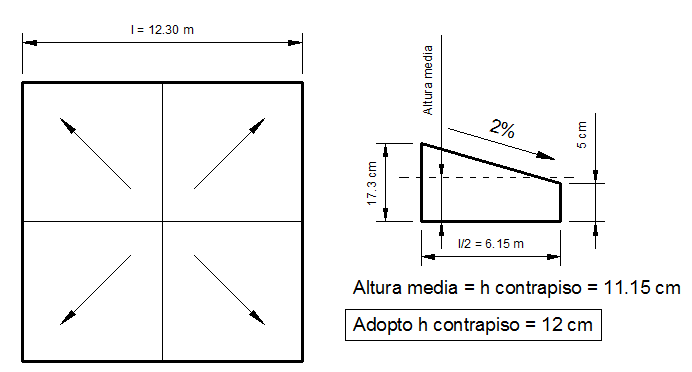
\includegraphics[scale = 0.8]{chapters/chapter_1/images/azotea.png}
\end{center}
\end{figure}
\begin{align*}
& \text{Peso propio} \rightarrow 0.14m \cdot 2500 \frac{Kg}{m^3} = 350 \frac{Kg}{m^2}\\
& \text{Contrapiso} \rightarrow 0.12m \cdot 1600 \frac{Kg}{m^3} = 192 \frac{Kg}{m^2}\\
& \text{Membrana + Aislación} \rightarrow = 20 \frac{Kg}{m^2}\\
& \text{Cielorraso aplicado} \rightarrow  0.02m \cdot 1300 \frac{Kg}{m^3} = 26 \frac{Kg}{m^2}\\
& D = 588 \frac{Kg}{m^2}\\
& L = 300 \frac{Kg}{m^2} \rightarrow \text{Según CIRSOC 101-05 - Capítulo 4}\\
& q_u = 1.2 \cdot D + 1.6 \cdot L = 1.2 \cdot 588 \frac{Kg}{m^2} + 1.6 \cdot 300 \frac{Kg}{m^2} = 1185.6 \frac{Kg}{m^2} \Rightarrow \framebox{$1.18 \frac{t}{m^2}$}\\
& q_u = 1.4 \cdot D = 1.4 \cdot 588 \frac{Kg}{m^2} = 823.2 \frac{Kg}{m^2} \Rightarrow 0.82 \frac{t}{m^2}
\end{align*}
\newpage
\item Losa L301: Azotea accesible privadamente

\begin{align*}
& \text{Peso propio} \rightarrow 0.14m \cdot 2500 \frac{Kg}{m^3} = 350 \frac{Kg}{m^2}\\
& \text{Contrapiso} \rightarrow 0.12m \cdot 1600 \frac{Kg}{m^3} = 192 \frac{Kg}{m^2}\\
& \text{Membrana + Aislación} \rightarrow = 20 \frac{Kg}{m^2}\\
& \text{Cielorraso aplicado} \rightarrow  0.02m \cdot 1300 \frac{Kg}{m^3} = 26 \frac{Kg}{m^2}\\
& D = 588 \frac{Kg}{m^2}\\
& D_{tanques} = \frac{2 \cdot 1100Kg + 2 \cdot 40Kg}{2 \cdot (\frac{\pi \cdot D^2}{4})}\\
& D_{tanques} = \frac{2 \cdot 1100Kg + 2 \cdot 40Kg}{2 \cdot (\frac{\pi \cdot (1.10m)^2}{4})}\\
& D_{tanques} = 1200 \frac{Kg}{m^2}\\
& L = 300 \frac{Kg}{m^2} \rightarrow \text{Según CIRSOC 101-05 - Capítulo 4}\\
& q_u = 1.2 \cdot D + 1.6 \cdot L = 1.2 \cdot 588 \frac{Kg}{m^2} + 1.6 \cdot 300 \frac{Kg}{m^2} = 1185.6 \frac{Kg}{m^2} \Rightarrow 1.18 \frac{t}{m^2}\\
& q_u = 1.4 \cdot (D + D_{tanques})= 1.4 \cdot (588 \frac{Kg}{m^2} + 1200 \frac{Kg}{m^2})= 2503.2 \frac{Kg}{m^2} \Rightarrow \framebox{$2.50 \frac{t}{m^2}$}
\end{align*}

\item Dpared Losa L108
\begin{align*}
& Dpared = \frac{(0.10m \cdot 2.6m \cdot 2.7m \cdot 1700 \frac{Kg}{m^3}) \cdot 1.50}{3.90m \cdot 5.20m} + \frac{(0.10m \cdot 1.10m \cdot 2.7m \cdot 1700 \frac{Kg}{m^3}) \cdot 1.70}{3.90m \cdot 5.20m}\\
& Dpared = 130.6 \frac{Kg}{m^2}
\end{align*}

\item Dpared Losa L110
\begin{align*}
& Dpared = (0.10m \cdot 2.7m \cdot 1700 \frac{Kg}{m^3}) \\
& Dpared = 459 \frac{Kg}{m}
\end{align*}
Consideramos la pared ocupando todo el ancho de la losa en una dirección.

\item Dpared Losa L202
\begin{align*}
& Dpared = (0.10m \cdot 1m \cdot 2.7m \cdot 1700 \frac{Kg}{m^3}) \\
& Dpared = 459Kg
\end{align*}

\item Dpared Losa L211
\begin{align*}
& Dpared = \frac{(0.10m \cdot (1m+1m+2.28) \cdot 2.7m \cdot 1700 \frac{Kg}{m^3}) \cdot 1.60}{3.60m \cdot 3.60m}\\
& + \frac{(0.10m \cdot 1.81m \cdot 2.7m \cdot 1700 \frac{Kg}{m^3}) \cdot 1.60}{3.60m \cdot 3.60m}\\
& Dpared = 345 \frac{Kg}{m^2}
\end{align*}

\item Dtanques Losa L301
\begin{align*}
& Dtanque = \frac{2 \cdot 1100Kg + 2 \cdot 40Kg}{2 \cdot (\frac{\pi \cdot D^2}{4})} \\
& Dtanque = \frac{2 \cdot 1100Kg + 2 \cdot 40Kg}{2 \cdot (\frac{\pi \cdot (1.10m)^2}{4})} \\
& Dtanque = 1200 \frac{Kg}{m^2}
\end{align*}
\end{itemize}

\item \underline{Momentos flectores - Nivel 1}\\
\begin{itemize}
\item Losa L101: Sala de Reuniones

\begin{figure}[H]
\begin{center}
     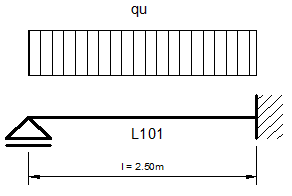
\includegraphics[scale = 0.8]{chapters/chapter_1/images/l101.png}
\end{center}
\end{figure}
\begin{align*}
& D = 528 \frac{Kg}{m^2}\\
& L = 500 \frac{Kg}{m^2} \rightarrow \text{Según CIRSOC 101-05 - Capítulo 4}\\
& q_u = 1.2 \cdot D + 1.6 \cdot L = 1.2 \cdot 528 \frac{Kg}{m^2} + 1.6 \cdot 500 \frac{Kg}{m^2} = 1433.6 \frac{Kg}{m^2} \Rightarrow \framebox{$1.43 \frac{t}{m^2}$} \\
& q_u = 1.4 \cdot D = 1.4 \cdot 528 \frac{Kg}{m^2} = 739.2 \frac{Kg}{m^2} \Rightarrow 0.739 \frac{t}{m^2}\\
& Mu_{empotrado} = \frac{q_u \cdot l^2}{8} = \frac{1.43 \frac{t}{m^2} \cdot (2.50m)^2}{8} = \framebox{$1.11 \frac{t \cdot m}{m}$}\\
& Mu_{tramo} = \frac{9}{128} \cdot q \cdot l^2 = \frac{9}{128} \cdot 1.43 \frac{t}{m^2} \cdot (2.50m)^2 = \framebox{$0.62 \frac{t \cdot m}{m}$}
\end{align*}
\newpage
\item Losa L102: Sala de Reuniones

\begin{figure}[H]
\begin{center}
     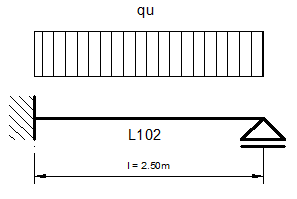
\includegraphics[scale = 0.8]{chapters/chapter_1/images/l102.png}
\end{center}
\end{figure}
\begin{align*}
& D = 528 \frac{Kg}{m^2}\\
& L = 500 \frac{Kg}{m^2} \rightarrow \text{Según CIRSOC 101-05 - Capítulo 4}\\
& q_u = 1.2 \cdot D + 1.6 \cdot L = 1.2 \cdot 528 \frac{Kg}{m^2} + 1.6 \cdot 500 \frac{Kg}{m^2} = 1433.6 \frac{Kg}{m^2} \Rightarrow \framebox{$1.43 \frac{t}{m^2}$} \\
& q_u = 1.4 \cdot D = 1.4 \cdot 528 \frac{Kg}{m^2} = 739.2 \frac{Kg}{m^2} \Rightarrow 0.739 \frac{t}{m^2}\\
& Mu_{empotrado} = \frac{q_u \cdot l^2}{8} = \frac{1.43 \frac{t}{m^2} \cdot (2.50m)^2}{8} = \framebox{$1.11 \frac{t \cdot m}{m}$}\\
& Mu_{tramo} = \frac{9}{128} \cdot q \cdot l^2 = \frac{9}{128} \cdot 1.43 \frac{t}{m^2} \cdot (2.50m)^2 = \framebox{$0.62 \frac{t \cdot m}{m}$}
\end{align*}

\item Losa L103: Balcón

\begin{figure}[H]
\begin{center}
     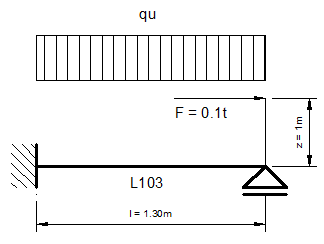
\includegraphics[scale = 0.8]{chapters/chapter_1/images/l103.png}
\end{center}
\end{figure}
\begin{align*}
& D = 528 \frac{Kg}{m^2}\\
& L = 500 \frac{Kg}{m^2} \rightarrow \text{Según CIRSOC 101-05 - Capítulo 4}\\
& q_u = 1.2 \cdot D + 1.6 \cdot L = 1.2 \cdot 528 \frac{Kg}{m^2} + 1.6 \cdot 500 \frac{Kg}{m^2} = 1433.6 \frac{Kg}{m^2} \Rightarrow \framebox{$1.43 \frac{t}{m^2}$} \\
& q_u = 1.4 \cdot D = 1.4 \cdot 528 \frac{Kg}{m^2} = 739.2 \frac{Kg}{m^2} \Rightarrow 0.739 \frac{t}{m^2}\\
& Mu_{empotrado} = \frac{q_u \cdot l^2}{2} + F \cdot z = \frac{1.43 \frac{t}{m^2} \cdot (1.30m)^2}{2} + 0.1t \cdot 1m = \framebox{$1.30 \frac{t \cdot m}{m}$}\\
\end{align*}

\item Losa L104: Recepción

\begin{figure}[H]
\begin{center}
     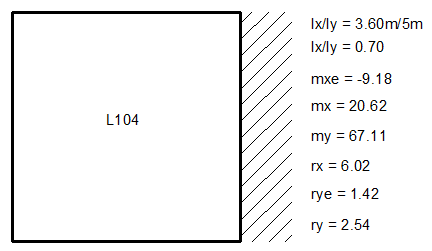
\includegraphics[scale = 0.8]{chapters/chapter_1/images/l104.png}
\end{center}
\end{figure}
\begin{align*}
& D = 528 \frac{Kg}{m^2}\\
& L = 250 \frac{Kg}{m^2} \rightarrow \text{Según CIRSOC 101-05 - Capítulo 4}\\
& q_u = 1.2 \cdot D + 1.6 \cdot L = 1.2 \cdot 528 \frac{Kg}{m^2} + 1.6 \cdot 250 \frac{Kg}{m^2} = 1033.3 \frac{Kg}{m^2} \Rightarrow \framebox{$1.03 \frac{t}{m^2}$} \\
& q_u = 1.4 \cdot D = 1.4 \cdot 528 \frac{Kg}{m^2} = 739.2 \frac{Kg}{m^2} \Rightarrow 0.739 \frac{t}{m^2} \\
& Mu_{xe} = \frac{q_u \cdot (l_{menor})^2}{m_{xe}} = \frac{1.03 \frac{t}{m^2} \cdot (3.60m)^2}{9.18} \framebox{$1.45 \frac{t \cdot m}{m}$}\\
& Mu_x = \frac{q_u \cdot (l_{menor})^2}{m_{x}} = \frac{1.03 \frac{t}{m^2} \cdot (3.60m)^2}{20.62} \framebox{$0.64 \frac{t \cdot m}{m}$}\\
& Mu_y = \frac{q_u \cdot (l_{menor})^2}{m_{y}} = \frac{1.03 \frac{t}{m^2} \cdot (3.60m)^2}{67.11} \framebox{$0.19 \frac{t \cdot m}{m}$}
\end{align*}
\newpage
\item Losa L105: Pasillo - Corredor

\begin{figure}[H]
\begin{center}
     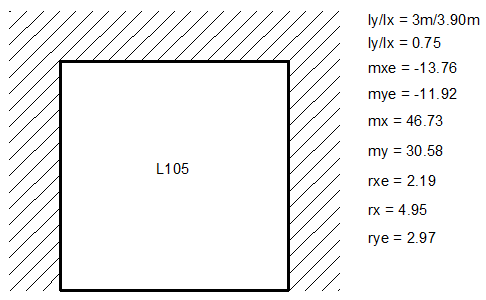
\includegraphics[scale = 0.8]{chapters/chapter_1/images/l105.png}
\end{center}
\end{figure}
\begin{align*}
& D = 528 \frac{Kg}{m^2}\\
& L = 400 \frac{Kg}{m^2} \rightarrow \text{Según CIRSOC 101-05 - Capítulo 4}\\
& q_u = 1.2 \cdot D + 1.6 \cdot L = 1.2 \cdot 528 \frac{Kg}{m^2} + 1.6 \cdot 400 \frac{Kg}{m^2} = 1273 \frac{Kg}{m^2} \Rightarrow \framebox{$1.27 \frac{t}{m^2}$} \\
& q_u = 1.4 \cdot D = 1.4 \cdot 528 \frac{Kg}{m^2} = 739.2 \frac{Kg}{m^2} \Rightarrow 0.739 \frac{t}{m^2} \\
& Mu_{xe} = \frac{q_u \cdot (l_{menor})^2}{m_{xe}} = \frac{1.27 \frac{t}{m^2} \cdot (3m)^2}{13.76} \framebox{$0.83 \frac{t \cdot m}{m}$}\\
& Mu_{ye} = \frac{q_u \cdot (l_{menor})^2}{m_{ye}} = \frac{1.27 \frac{t}{m^2} \cdot (3m)^2}{11.92} \framebox{$0.96 \frac{t \cdot m}{m}$}\\
& Mu_x = \frac{q_u \cdot (l_{menor})^2}{m_{x}} = \frac{1.27 \frac{t}{m^2} \cdot (3m)^2}{46.73} \framebox{$0.83 \frac{t \cdot m}{m}$}\\
& Mu_y = \frac{q_u \cdot (l_{menor})^2}{m_{y}} = \frac{1.27 \frac{t}{m^2} \cdot (3m)^2}{30.58} \framebox{$0.37 \frac{t \cdot m}{m}$}
\end{align*}
\newpage
\item Losa L106: Aula

\begin{figure}[H]
\begin{center}
     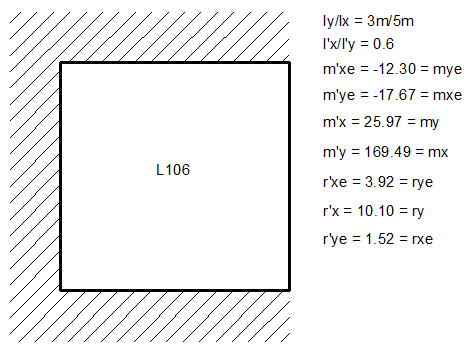
\includegraphics[scale = 0.8]{chapters/chapter_1/images/l106.png}
\end{center}
\end{figure}
\begin{align*}
& D = 528 \frac{Kg}{m^2}\\
& L = 300 \frac{Kg}{m^2} \rightarrow \text{Según CIRSOC 101-05 - Capítulo 4}\\
& q_u = 1.2 \cdot D + 1.6 \cdot L = 1.2 \cdot 528 \frac{Kg}{m^2} + 1.6 \cdot 300 \frac{Kg}{m^2} = 1113.6 \frac{Kg}{m^2} \Rightarrow \framebox{$1.11 \frac{t}{m^2}$} \\
& q_u = 1.4 \cdot D = 1.4 \cdot 528 \frac{Kg}{m^2} = 739.2 \frac{Kg}{m^2} \Rightarrow 0.739 \frac{t}{m^2}\\
& Mu_{xe} = \frac{q_u \cdot (l_{menor})^2}{m_{xe}} = \frac{1.11 \frac{t}{m^2} \cdot (3m)^2}{17.67} \framebox{$0.56 \frac{t \cdot m}{m}$}\\
& Mu_{ye} = \frac{q_u \cdot (l_{menor})^2}{m_{ye}} = \frac{1.11 \frac{t}{m^2} \cdot (3m)^2}{12.30} \framebox{$0.81 \frac{t \cdot m}{m}$}\\
& Mu_x = \frac{q_u \cdot (l_{menor})^2}{m_{x}} = \frac{1.11 \frac{t}{m^2} \cdot (3m)^2}{169.49} \framebox{$0.058 \frac{t \cdot m}{m}$}\\
& Mu_y = \frac{q_u \cdot (l_{menor})^2}{m_{y}} = \frac{1.11 \frac{t}{m^2} \cdot (3m)^2}{25.97} \framebox{$0.38 \frac{t \cdot m}{m}$}
\end{align*}
\newpage
\item Losa L107: Pasillo - Corredor

\begin{figure}[H]
\begin{center}
     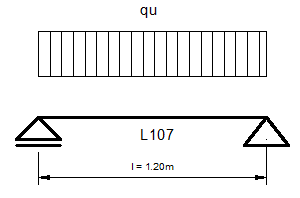
\includegraphics[scale = 0.8]{chapters/chapter_1/images/l107.png}
\end{center}
\end{figure}
\begin{align*}
& D = 528 \frac{Kg}{m^2}\\
& L = 400 \frac{Kg}{m^2} \rightarrow \text{Según CIRSOC 101-05 - Capítulo 4}\\
& q_u = 1.2 \cdot D + 1.6 \cdot L = 1.2 \cdot 528 \frac{Kg}{m^2} + 1.6 \cdot 400 \frac{Kg}{m^2} = 1273 \frac{Kg}{m^2} \Rightarrow \framebox{$1.27 \frac{t}{m^2}$} \\
& q_u = 1.4 \cdot D = 1.4 \cdot 528 \frac{Kg}{m^2} = 739.2 \frac{Kg}{m^2} \Rightarrow 0.739 \frac{t}{m^2} \\
& Mu_{tramo} = \frac{q_u \cdot l^2}{8} = \frac{1.27 \frac{t}{m^2} \cdot (1.20m)^2}{8} = \framebox{$0.23 \frac{t \cdot m}{m}$}
\end{align*}
\newpage
\item Losa L108: Aula

\begin{figure}[H]
\begin{center}
     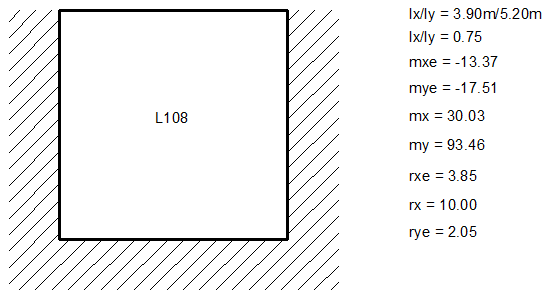
\includegraphics[scale = 0.8]{chapters/chapter_1/images/l108_bis.png}
\end{center}
\end{figure}
\begin{align*}
& D = 528 \frac{Kg}{m^2}\\
& Dpared = 130.6 \frac{Kg}{m^2}\\
& Dtotal = 528 \frac{Kg}{m^2} + 130.6 \frac{Kg}{m^2} = 658.6 \frac{Kg}{m^2}\\\\
& L = 300 \frac{Kg}{m^2} \rightarrow \text{Según CIRSOC 101-05 - Capítulo 4}\\
& q_u = 1.2 \cdot Dtotal + 1.6 \cdot L = 1.2 \cdot 658.6 \frac{Kg}{m^2} + 1.6 \cdot 300 \frac{Kg}{m^2} = 1270.32 \frac{Kg}{m^2} \Rightarrow \framebox{$1.27 \frac{t}{m^2}$} \\
& q_u = 1.4 \cdot Dtotal = 1.4 \cdot 658.6 \frac{Kg}{m^2} = 922.04 \frac{Kg}{m^2} \Rightarrow 0.92 \frac{t}{m^2}\\
& Mu_{xe} = \frac{q_u \cdot (l_{menor})^2}{m_{xe}} = \frac{1.27 \frac{t}{m^2} \cdot (3.90m)^2}{13.37} \framebox{$1.44 \frac{t \cdot m}{m}$}\\
& Mu_{ye} = \frac{q_u \cdot (l_{menor})^2}{m_{ye}} = \frac{1.27 \frac{t}{m^2} \cdot (3.90m)^2}{17.51} \framebox{$1.10 \frac{t \cdot m}{m}$}\\
& Mu_x = \frac{q_u \cdot (l_{menor})^2}{m_{x}} = \frac{1.27 \frac{t}{m^2} \cdot (3.90m)^2}{30.03} \framebox{$0.64 \frac{t \cdot m}{m}$}\\
& Mu_y = \frac{q_u \cdot (l_{menor})^2}{m_{y}} = \frac{1.27 \frac{t}{m^2} \cdot (3.90m)^2}{93.46} \framebox{$0.20 \frac{t \cdot m}{m}$}
\end{align*}

Debido a que la losa L108 no es compatible con la losa L109 es que analizamos la siguiente sustentación.\\

\begin{figure}[H]
\begin{center}
     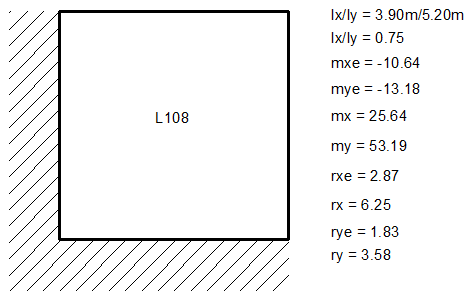
\includegraphics[scale = 0.8]{chapters/chapter_1/images/l108.png}
\end{center}
\end{figure}
\begin{align*}
& D = 528 \frac{Kg}{m^2}\\
& Dpared = 130.6 \frac{Kg}{m^2}\\
& Dtotal = 528 \frac{Kg}{m^2} + 130.6 \frac{Kg}{m^2} = 658.6 \frac{Kg}{m^2}\\\\
& L = 300 \frac{Kg}{m^2} \rightarrow \text{Según CIRSOC 101-05 - Capítulo 4}\\
& q_u = 1.2 \cdot Dtotal + 1.6 \cdot L = 1.2 \cdot 658.6 \frac{Kg}{m^2} + 1.6 \cdot 300 \frac{Kg}{m^2} = 1270.32 \frac{Kg}{m^2} \Rightarrow \framebox{$1.27 \frac{t}{m^2}$} \\
& q_u = 1.4 \cdot Dtotal = 1.4 \cdot 658.6 \frac{Kg}{m^2} = 922.04 \frac{Kg}{m^2} \Rightarrow 0.92 \frac{t}{m^2}\\
& Mu_{xe} = \frac{q_u \cdot (l_{menor})^2}{m_{xe}} = \frac{1.27 \frac{t}{m^2} \cdot (3.90m)^2}{10.64} \framebox{$1.81 \frac{t \cdot m}{m}$}\\
& Mu_{ye} = \frac{q_u \cdot (l_{menor})^2}{m_{ye}} = \frac{1.27 \frac{t}{m^2} \cdot (3.90m)^2}{13.18} \framebox{$1.46 \frac{t \cdot m}{m}$}\\
& Mu_x = \frac{q_u \cdot (l_{menor})^2}{m_{x}} = \frac{1.27 \frac{t}{m^2} \cdot (3.90m)^2}{25.64} \framebox{$0.75 \frac{t \cdot m}{m}$}\\
& Mu_y = \frac{q_u \cdot (l_{menor})^2}{m_{y}} = \frac{1.27 \frac{t}{m^2} \cdot (3.90m)^2}{53.19} \framebox{$0.36 \frac{t \cdot m}{m}$}
\end{align*}
\newpage
\item Losa L109: Sala de Usos Múltiples

\begin{figure}[H]
\begin{center}
     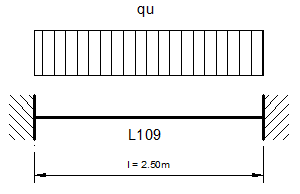
\includegraphics[scale = 0.8]{chapters/chapter_1/images/l109.png}
\end{center}
\end{figure}
\begin{align*}
& D = 528 \frac{Kg}{m^2}\\
& L = 500 \frac{Kg}{m^2} \rightarrow \text{Según CIRSOC 101-05 - Capítulo 4}\\
& q_u = 1.2 \cdot D + 1.6 \cdot L = 1.2 \cdot 528 \frac{Kg}{m^2} + 1.6 \cdot 500 \frac{Kg}{m^2} = 1433.6 \frac{Kg}{m^2} \Rightarrow \framebox{$1.43 \frac{t}{m^2}$} \\
& q_u = 1.4 \cdot D = 1.4 \cdot 528 \frac{Kg}{m^2} = 739.2 \frac{Kg}{m^2} \Rightarrow 0.739 \frac{t}{m^2}\\
& Mu_{empotrado} = \frac{q_u \cdot l^2}{12} = \frac{1.43 \frac{t}{m^2} \cdot (2.50m)^2}{12} = \framebox{$0.74 \frac{t \cdot m}{m}$}\\
& Mu_{tramo} = \frac{q_u \cdot l^2}{24} = \frac{1.43 \frac{t}{m^2} \cdot (2.50m)^2}{24} = \framebox{$0.37 \frac{t \cdot m}{m}$}
\end{align*}

\item Losa L110: Sala de Usos Múltiples

\begin{figure}[H]
\begin{center}
     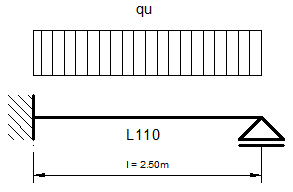
\includegraphics[scale = 0.8]{chapters/chapter_1/images/l110.png}
\end{center}
\end{figure}
\begin{align*}
& D = 528 \frac{Kg}{m^2}\\
& Dpared = 459 \frac{Kg}{m}\\
& Dtotal = 987 \frac{Kg}{m}\\
& L = 500 \frac{Kg}{m^2} \rightarrow \text{Según CIRSOC 101-05 - Capítulo 4}\\
& q_u = 1.2 \cdot D + 1.6 \cdot L = 1.2 \cdot 987 \frac{Kg}{m^2} + 1.6 \cdot 500 \frac{Kg}{m^2} = 1984.4 \frac{Kg}{m^2} \Rightarrow \framebox{$1.98 \frac{t}{m^2}$} \\
& q_u = 1.4 \cdot D = 1.4 \cdot 987 \frac{Kg}{m^2} = 1381.8 \frac{Kg}{m^2} \Rightarrow 1.38 \frac{t}{m^2}\\
& Mu_{empotrado} = \frac{q_u \cdot l^2}{8} = \frac{1.98 \frac{t}{m^2} \cdot (2.50m)^2}{8} = \framebox{$1.54 \frac{t \cdot m}{m}$}\\
& Mu_{tramo} = \frac{9}{128} \cdot q \cdot l^2 = \frac{9}{128} \cdot 1.98 \frac{t}{m^2} \cdot (2.50m)^2 = \framebox{$0.87 \frac{t \cdot m}{m}$}
\end{align*}

\item Losa L111: Baños

\begin{figure}[H]
\begin{center}
     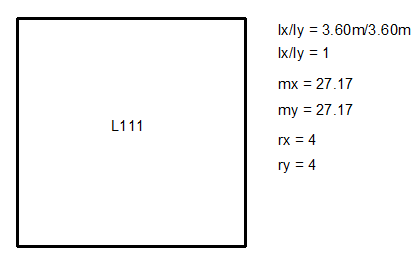
\includegraphics[scale = 0.8]{chapters/chapter_1/images/l111.png}
\end{center}
\end{figure}
\begin{align*}
& D = 858 \frac{Kg}{m^2}\\
& L = 300 \frac{Kg}{m^2} \rightarrow \text{Según CIRSOC 101-05 - Capítulo 4}\\
& q_u = 1.2 \cdot D + 1.6 \cdot L = 1.2 \cdot 858 \frac{Kg}{m^2} + 1.6 \cdot 300 \frac{Kg}{m^2} = 1509.6 \frac{Kg}{m^2} \Rightarrow \framebox{$1.50 \frac{t}{m^2}$}\\
& q_u = 1.4 \cdot D = 1.4 \cdot 858 \frac{Kg}{m^2} = 1201.2 \frac{Kg}{m^2} \Rightarrow 1.20 \frac{t}{m^2}\\
& Mu_x = Mu_y = \frac{q_u \cdot l^2}{m_{x}} = \frac{1.50 \frac{t}{m^2} \cdot (3.60m)^2}{27.17} \framebox{$0.71 \frac{t \cdot m}{m}$}\\
\end{align*}
\end{itemize}
\newpage
\item \underline{Compatibilización de Momentos - Nivel 1}\\

\begin{itemize}
\item Losas L104 y L108
\begin{align*}
& (1.81-1.45) < 0.40 \cdot \frac{(1.81+1.45)}{2}\\
& 0.36 < 0.65 \Rightarrow \quad \text{Verifica}\\
& \text{Adopto} \quad \framebox{1.62} \quad \text{en el apoyo}\\
& 0.75 + (1.81-1.62) = 0.93\\
& \text{Adopto} \quad \framebox{0.93} \quad \text{en el tramo}\\
\end{align*}

\item Losas L105 y L108
\begin{align*}
& (1.46-0.96) < 0.40 \cdot \frac{(1.46+0.96)}{2}\\
& 0.5 < 0.48 \Rightarrow \quad \text{No Verifica}\\
& \text{Adopto de todas formas} \quad \framebox{1.21} \quad \text{en el apoyo}\\
& 0.36 + (1.46-1.21) = 0.61\\
& \text{Adopto} \quad \framebox{0.61} \quad \text{en el tramo}\\
\end{align*}

\item Losas L105 y L106
\begin{align*}
& (0.83-0.56) < 0.40 \cdot \frac{(0.83+0.56)}{2}\\
& 0.27 < 0.278 \Rightarrow \quad \text{Verifica}\\
& \text{Adopto} \quad \framebox{0.69} \quad \text{en el apoyo}\\
& 0.24 + (0.83-0.69) = 0.38\\
& \text{Adopto} \quad \framebox{0.38} \quad \text{en el tramo}\\
\end{align*}

\item Losas L109 y L110
\begin{align*}
& \frac{(0.74+1.54)}{2} = 1.14\\
& \text{Adopto} \quad \framebox{1.14} \quad \text{en el apoyo}\\
& 0.87 + (1.54-1.14) = 1.27\\
& \text{Adopto} \quad \framebox{1.27} \quad \text{en el tramo}\\
\end{align*}
\end{itemize}
\newpage
\item \underline{Momentos flectores - Nivel 2}\\
\begin{itemize}
\item Losa L201: Aulas

\begin{figure}[H]
\begin{center}
     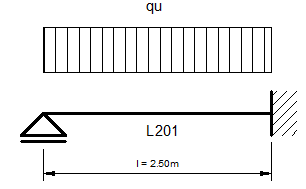
\includegraphics[scale = 0.8]{chapters/chapter_1/images/l201.png}
\end{center}
\end{figure}
\begin{align*}
& D = 528 \frac{Kg}{m^2}\\
& L = 300 \frac{Kg}{m^2} \rightarrow \text{Según CIRSOC 101-05 - Capítulo 4}\\
& q_u = 1.2 \cdot D + 1.6 \cdot L = 1.2 \cdot 528 \frac{Kg}{m^2} + 1.6 \cdot 300 \frac{Kg}{m^2} = 1113.6 \frac{Kg}{m^2} \Rightarrow \framebox{$1.11 \frac{t}{m^2}$} \\
& q_u = 1.4 \cdot D = 1.4 \cdot 528 \frac{Kg}{m^2} = 739.2 \frac{Kg}{m^2} \Rightarrow 0.739 \frac{t}{m^2}\\
& Mu_{apoyo} = \frac{q_u \cdot l^2}{8} = \frac{1.11 \frac{t}{m^2} \cdot (2.50m)^2}{8} = \framebox{$0.86 \frac{t \cdot m}{m}$}\\
& Mu_{tramo} = \frac{9}{128} \cdot q \cdot l^2 = \frac{9}{128} \cdot 1.11 \frac{t}{m^2} \cdot (2.50m)^2 = \framebox{$0.48 \frac{t \cdot m}{m}$}
\end{align*}
\newpage
\item Losa L202: Aulas

\begin{figure}[H]
\begin{center}
     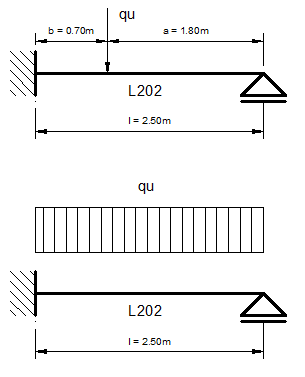
\includegraphics[scale = 0.8]{chapters/chapter_1/images/l202.png}
\end{center}
\end{figure}
\begin{align*}
& D = 528 \frac{Kg}{m^2}\\
& Dpared = 459 Kg\\
& L = 300 \frac{Kg}{m^2} \rightarrow \text{Según CIRSOC 101-05 - Capítulo 4}\\
& q_u = 1.2 \cdot D + 1.6 \cdot L = 1.2 \cdot 528 \frac{Kg}{m^2} + 1.6 \cdot 300 \frac{Kg}{m^2} = 1113.6 \frac{Kg}{m^2} \Rightarrow \framebox{$1.11 \frac{t}{m^2}$} \\
& q_u = 1.4 \cdot D = 1.4 \cdot 528 \frac{Kg}{m^2} = 739.2 \frac{Kg}{m^2} \Rightarrow 0.739 \frac{t}{m^2}\\
& q_u = 1.2 \cdot Dpared = 1.2 \cdot 459Kg = 550.8Kg \Rightarrow 0.55t\\
& \text{Carga uniformemente ditribuída:}\\
& Mu_{empotrado} = \frac{q_u \cdot l^2}{8} = \frac{1.11 \frac{t}{m^2} \cdot (2.50m)^2}{8} = \framebox{$0.86 \frac{t \cdot m}{m}$}\\
& Mu_{tramo} = \frac{9}{128} \cdot q \cdot l^2 = \frac{9}{128} \cdot 1.11 \frac{t}{m^2} \cdot (2.50m)^2 = \framebox{$0.48 \frac{t \cdot m}{m}$}\\
& \text{Carga concentrada:}\\
& Mu_{empotrado} = \frac{q_u \cdot a}{2 \cdot l^2} \cdot (l^2-a^2)= \frac{0.55t \cdot 1.80m}{2 \cdot (2.50m)^2} \cdot ((2.50m)^2-(1.80m)^2) = \framebox{$0.23 \frac{t \cdot m}{m}$}\\
& Mu_{tramo} = \frac{q_u \cdot a}{2 \cdot l^3} \cdot b^2 \cdot (3 \cdot a+2 \cdot b)\\
& Mu_{tramo} = \frac{0.55t \cdot 1.80m}{2 \cdot (2.50m)^3} \cdot (0.70m)^2 \cdot (3 \cdot 1.80m + 2 \cdot 0.70m)=\framebox{$0.10 \frac{t \cdot m}{m}$}\\
& \text{Superposición de efectos:}\\
& Mu_{empotrado} = \framebox{$0.86 \frac{t \cdot m}{m}$}\\
& Mu_{tramo} = 0.48 \frac{t \cdot m}{m}+0.10 \frac{t \cdot m}{m} = \framebox{$0.58 \frac{t \cdot m}{m}$}
\end{align*}
\newpage
\item Losa L203: Balcón

\begin{figure}[H]
\begin{center}
     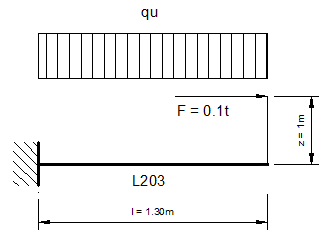
\includegraphics[scale = 0.8]{chapters/chapter_1/images/l203.png}
\end{center}
\end{figure}
\begin{align*}
& D = 528 \frac{Kg}{m^2}\\
& L = 500 \frac{Kg}{m^2} \rightarrow \text{Según CIRSOC 101-05 - Capítulo 4}\\
& q_u = 1.2 \cdot D + 1.6 \cdot L = 1.2 \cdot 528 \frac{Kg}{m^2} + 1.6 \cdot 500 \frac{Kg}{m^2} = 1433.6 \frac{Kg}{m^2} \Rightarrow \framebox{$1.43 \frac{t}{m^2}$} \\
& q_u = 1.4 \cdot D = 1.4 \cdot 528 \frac{Kg}{m^2} = 739.2 \frac{Kg}{m^2} \Rightarrow 0.739 \frac{t}{m^2}\\
& Mu_{empotrado} = \frac{q_u \cdot l^2}{2} + F \cdot z = \frac{1.43 \frac{t}{m^2} \cdot (1.30m)^2}{2} + 0.1t \cdot 1m = \framebox{$1.30 \frac{t \cdot m}{m}$}\\
\end{align*}
\newpage
\item Losa L204: Cocina - Comedor

\begin{figure}[H]
\begin{center}
     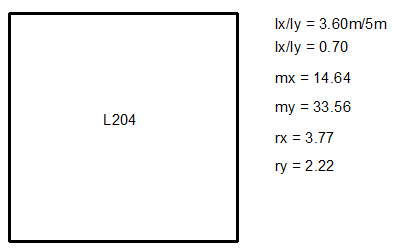
\includegraphics[scale = 0.8]{chapters/chapter_1/images/l204.png}
\end{center}
\end{figure}
\begin{align*}
& D = 858 \frac{Kg}{m^2}\\
& L = 500 \frac{Kg}{m^2} \rightarrow \text{Según CIRSOC 101-05 - Capítulo 4}\\
& q_u = 1.2 \cdot D + 1.6 \cdot L = 1.2 \cdot 858 \frac{Kg}{m^2} + 1.6 \cdot 500 \frac{Kg}{m^2} = 1829.6 \frac{Kg}{m^2} \Rightarrow \framebox{$1.82 \frac{t}{m^2}$}\\
& q_u = 1.4 \cdot D = 1.4 \cdot 858 \frac{Kg}{m^2} = 1201.2 \frac{Kg}{m^2} \Rightarrow 1.20 \frac{t}{m^2} \\
& Mu_x = \frac{q_u \cdot (l_{menor})^2}{m_{x}} = \frac{1.82 \frac{t}{m^2} \cdot (3.60m)^2}{14.64} \framebox{$1.61 \frac{t \cdot m}{m}$}\\
& Mu_y = \frac{q_u \cdot (l_{menor})^2}{m_{y}} = \frac{1.82 \frac{t}{m^2} \cdot (3.60m)^2}{33.56} \framebox{$0.70 \frac{t \cdot m}{m}$}
\end{align*}
\newpage
\item Losa L205: Pasillo - Corredor

\begin{figure}[H]
\begin{center}
     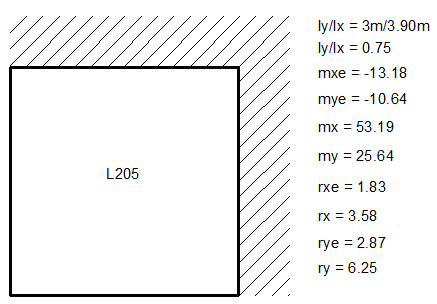
\includegraphics[scale = 0.8]{chapters/chapter_1/images/l205.png}
\end{center}
\end{figure}
\begin{align*}
& D = 528 \frac{Kg}{m^2}\\
& L = 400 \frac{Kg}{m^2} \rightarrow \text{Según CIRSOC 101-05 - Capítulo 4}\\
& q_u = 1.2 \cdot D + 1.6 \cdot L = 1.2 \cdot 528 \frac{Kg}{m^2} + 1.6 \cdot 400 \frac{Kg}{m^2} = 1273 \frac{Kg}{m^2} \Rightarrow \framebox{$1.27 \frac{t}{m^2}$} \\
& q_u = 1.4 \cdot D = 1.4 \cdot 528 \frac{Kg}{m^2} = 739.2 \frac{Kg}{m^2} \Rightarrow 0.739 \frac{t}{m^2} \\
& Mu_{xe} = \frac{q_u \cdot (l_{menor})^2}{m_{xe}} = \frac{1.27 \frac{t}{m^2} \cdot (3m)^2}{13.18} \framebox{$0.86 \frac{t \cdot m}{m}$}\\
& Mu_{ye} = \frac{q_u \cdot (l_{menor})^2}{m_{ye}} = \frac{1.27 \frac{t}{m^2} \cdot (3m)^2}{10.64} \framebox{$1.07 \frac{t \cdot m}{m}$}\\
& Mu_x = \frac{q_u \cdot (l_{menor})^2}{m_{x}} = \frac{1.27 \frac{t}{m^2} \cdot (3m)^2}{53.19} \framebox{$0.21 \frac{t \cdot m}{m}$}\\
& Mu_y = \frac{q_u \cdot (l_{menor})^2}{m_{y}} = \frac{1.27 \frac{t}{m^2} \cdot (3m)^2}{25.64} \framebox{$0.44 \frac{t \cdot m}{m}$}
\end{align*}
\newpage
\item Losa L206: Secretaria

\begin{figure}[H]
\begin{center}
     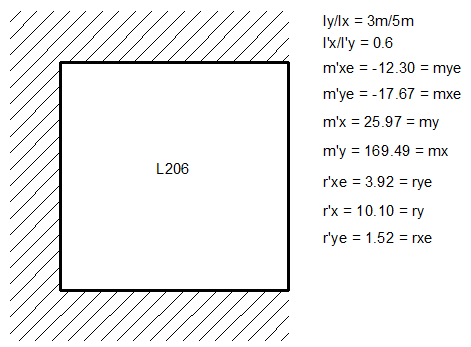
\includegraphics[scale = 0.8]{chapters/chapter_1/images/l206.png}
\end{center}
\end{figure}
\begin{align*}
& D = 528 \frac{Kg}{m^2}\\
& L = 250 \frac{Kg}{m^2} \rightarrow \text{Según CIRSOC 101-05 - Capítulo 4}\\
& q_u = 1.2 \cdot D + 1.6 \cdot L = 1.2 \cdot 528 \frac{Kg}{m^2} + 1.6 \cdot 250 \frac{Kg}{m^2} = 1033.3 \frac{Kg}{m^2} \Rightarrow \framebox{$1.03 \frac{t}{m^2}$} \\
& q_u = 1.4 \cdot D = 1.4 \cdot 528 \frac{Kg}{m^2} = 739.2 \frac{Kg}{m^2} \Rightarrow 0.739 \frac{t}{m^2}\\
& Mu_{xe} = \frac{q_u \cdot (l_{menor})^2}{m_{xe}} = \frac{1.03 \frac{t}{m^2} \cdot (3m)^2}{17.67} \framebox{$0.52 \frac{t \cdot m}{m}$}\\
& Mu_{ye} = \frac{q_u \cdot (l_{menor})^2}{m_{ye}} = \frac{1.03 \frac{t}{m^2} \cdot (3m)^2}{12.30} \framebox{$0.75 \frac{t \cdot m}{m}$}\\
& Mu_x = \frac{q_u \cdot (l_{menor})^2}{m_{x}} = \frac{1.03 \frac{t}{m^2} \cdot (3m)^2}{169.49} \framebox{$0.054 \frac{t \cdot m}{m}$}\\
& Mu_y = \frac{q_u \cdot (l_{menor})^2}{m_{y}} = \frac{1.03 \frac{t}{m^2} \cdot (3m)^2}{25.97} \framebox{$0.35 \frac{t \cdot m}{m}$}
\end{align*}

\item Losa L207: Pasillo - Corredor

\begin{figure}[H]
\begin{center}
     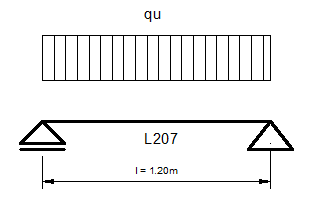
\includegraphics[scale = 0.8]{chapters/chapter_1/images/l207.png}
\end{center}
\end{figure}
\begin{align*}
& D = 528 \frac{Kg}{m^2}\\
& L = 400 \frac{Kg}{m^2} \rightarrow \text{Según CIRSOC 101-05 - Capítulo 4}\\
& q_u = 1.2 \cdot D + 1.6 \cdot L = 1.2 \cdot 528 \frac{Kg}{m^2} + 1.6 \cdot 400 \frac{Kg}{m^2} = 1273 \frac{Kg}{m^2} \Rightarrow \framebox{$1.27 \frac{t}{m^2}$} \\
& q_u = 1.4 \cdot D = 1.4 \cdot 528 \frac{Kg}{m^2} = 739.2 \frac{Kg}{m^2} \Rightarrow 0.739 \frac{t}{m^2} \\
& Mu_{tramo} = \frac{q_u \cdot l^2}{8} = \frac{1.27 \frac{t}{m^2} \cdot (1.20m)^2}{8} = \framebox{$0.23 \frac{t \cdot m}{m}$}
\end{align*}

\item Losa L208: Aulas

\begin{figure}[H]
\begin{center}
     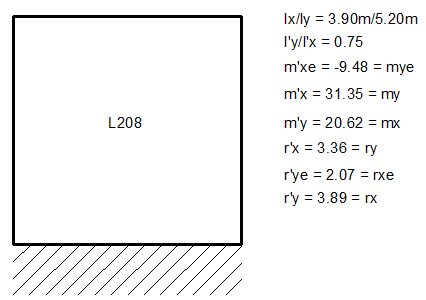
\includegraphics[scale = 0.8]{chapters/chapter_1/images/l208.png}
\end{center}
\end{figure}
\begin{align*}
& D = 528 \frac{Kg}{m^2}\\
& L = 300 \frac{Kg}{m^2} \rightarrow \text{Según CIRSOC 101-05 - Capítulo 4}\\
& q_u = 1.2 \cdot D + 1.6 \cdot L = 1.2 \cdot 528 \frac{Kg}{m^2} + 1.6 \cdot 300 \frac{Kg}{m^2} = 1113.6 \frac{Kg}{m^2} \Rightarrow \framebox{$1.11 \frac{t}{m^2}$} \\
& q_u = 1.4 \cdot D = 1.4 \cdot 528 \frac{Kg}{m^2} = 739.2 \frac{Kg}{m^2} \Rightarrow 0.739 \frac{t}{m^2}\\
& Mu_{ye} = \frac{q_u \cdot (l_{menor})^2}{m_{ye}} = \frac{1.11 \frac{t}{m^2} \cdot (3.90m)^2}{9.48} \framebox{$1.78 \frac{t \cdot m}{m}$}\\
& Mu_x = \frac{q_u \cdot (l_{menor})^2}{m_{x}} = \frac{1.11 \frac{t}{m^2} \cdot (3.90m)^2}{20.62} \framebox{$0.81 \frac{t \cdot m}{m}$}\\
& Mu_y = \frac{q_u \cdot (l_{menor})^2}{m_{y}} = \frac{1.11 \frac{t}{m^2} \cdot (3.90m)^2}{31.35} \framebox{$0.53 \frac{t \cdot m}{m}$}
\end{align*}
\newpage
\item Losa L209: Aulas

\begin{figure}[H]
\begin{center}
     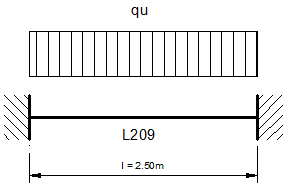
\includegraphics[scale = 0.8]{chapters/chapter_1/images/l209.png}
\end{center}
\end{figure}
\begin{align*}
& D = 528 \frac{Kg}{m^2}\\
& L = 300 \frac{Kg}{m^2} \rightarrow \text{Según CIRSOC 101-05 - Capítulo 4}\\
& q_u = 1.2 \cdot D + 1.6 \cdot L = 1.2 \cdot 528 \frac{Kg}{m^2} + 1.6 \cdot 300 \frac{Kg}{m^2} = 1113.6 \frac{Kg}{m^2} \Rightarrow \framebox{$1.11 \frac{t}{m^2}$} \\
& q_u = 1.4 \cdot D = 1.4 \cdot 528 \frac{Kg}{m^2} = 739.2 \frac{Kg}{m^2} \Rightarrow 0.739 \frac{t}{m^2}\\
& Mu_{empotrado} = \frac{q_u \cdot l^2}{12} = \frac{1.11 \frac{t}{m^2} \cdot (2.50m)^2}{12} = \framebox{$0.57 \frac{t \cdot m}{m}$}\\
& Mu_{tramo} = \frac{q_u \cdot l^2}{24} = \frac{1.11 \frac{t}{m^2} \cdot (2.50m)^2}{24} = \framebox{$0.28 \frac{t \cdot m}{m}$}
\end{align*}

\item Losa L210: Sala de Computación

\begin{figure}[H]
\begin{center}
     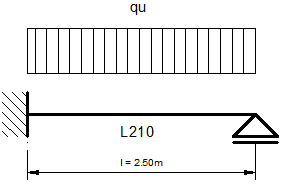
\includegraphics[scale = 0.8]{chapters/chapter_1/images/l210.png}
\end{center}
\end{figure}
\begin{align*}
& D = 528 \frac{Kg}{m^2}\\
& L = 500 \frac{Kg}{m^2} \rightarrow \text{Según CIRSOC 101-05 - Capítulo 4}\\
& q_u = 1.2 \cdot D + 1.6 \cdot L = 1.2 \cdot 528 \frac{Kg}{m^2} + 1.6 \cdot 500 \frac{Kg}{m^2} = 1433.6 \frac{Kg}{m^2} \Rightarrow \framebox{$1.43 \frac{t}{m^2}$} \\
& q_u = 1.4 \cdot D = 1.4 \cdot 528 \frac{Kg}{m^2} = 739.2 \frac{Kg}{m^2} \Rightarrow 0.739 \frac{t}{m^2}\\
& Mu_{empotrado} = \frac{q_u \cdot l^2}{8} = \frac{1.43 \frac{t}{m^2} \cdot (2.50m)^2}{8} = \framebox{$1.11 \frac{t \cdot m}{m}$}\\
& Mu_{tramo} = \frac{9}{128} \cdot q \cdot l^2 = \frac{9}{128} \cdot 1.43 \frac{t}{m^2} \cdot (2.50m)^2 = \framebox{$0.62 \frac{t \cdot m}{m}$}
\end{align*}

\item Losa L211: Baños

\begin{figure}[H]
\begin{center}
     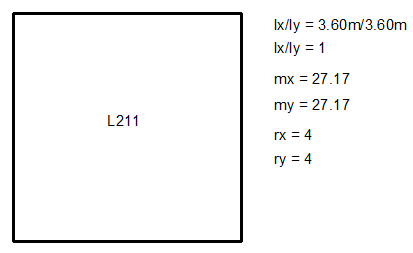
\includegraphics[scale = 0.8]{chapters/chapter_1/images/l211.png}
\end{center}
\end{figure}
\begin{align*}
& D = 858 \frac{Kg}{m^2}\\
& Dpared = 345 \frac{Kg}{m^2}\\
& Dtotal = 1203 \frac{Kg}{m^2}\\
& L = 300 \frac{Kg}{m^2} \rightarrow \text{Según CIRSOC 101-05 - Capítulo 4}\\
& q_u = 1.2 \cdot D + 1.6 \cdot L = 1.2 \cdot 1203 \frac{Kg}{m^2} + 1.6 \cdot 300 \frac{Kg}{m^2} = 1923.6 \frac{Kg}{m^2} \Rightarrow \framebox{$1.92 \frac{t}{m^2}$}\\
& q_u = 1.4 \cdot D = 1.4 \cdot 1203 \frac{Kg}{m^2} = 1684.2 \frac{Kg}{m^2} \Rightarrow 1.68 \frac{t}{m^2}\\
& Mu_x = Mu_y = \frac{q_u \cdot (l_{menor})^2}{m_{x}} = \frac{1.92 \frac{t}{m^2} \cdot (3.60m)^2}{27.17} \framebox{$0.91 \frac{t \cdot m}{m}$}\\
\end{align*}
\end{itemize}
\newpage
\item \underline{Compatibilización de Momentos - Nivel 2}\\

\begin{itemize}
\item Losas L205 y L208
\begin{align*}
& (1.78-1.07) < 0.40 \cdot \frac{(1.78+1.07)}{2}\\
& 0.71 < 0.57 \Rightarrow \quad \text{No Verifica}\\
& \text{Adopto} \quad \framebox{1.42} \quad \text{en el apoyo}\\
& 0.53 + (1.78-1.42) = 0.89\\
& \text{Adopto} \quad \framebox{0.89} \quad \text{en el tramo}\\
\end{align*}

\item Losas L205 y L206
\begin{align*}
& (0.86-0.52) < 0.40 \cdot \frac{(0.86+0.52)}{2}\\
& 0.34 < 0.28 \Rightarrow \quad \text{No Verifica}\\
& \text{Adopto} \quad \framebox{0.69} \quad \text{en el apoyo}\\
& 0.21 + (0.86-0.69) = 0.38\\
& \text{Adopto} \quad \framebox{0.38} \quad \text{en el tramo}\\
\end{align*}

\item Losas L209 y L210
\begin{align*}
& (1.11-0.57) < 0.40 \cdot \frac{(1.11+0.57)}{2}\\
& 0.54 < 0.33 \Rightarrow \quad \text{No Verifica}\\
& \text{Adopto} \quad \framebox{0.84} \quad \text{en el apoyo}\\
& 0.62 + (1.11-0.84) = 0.89\\
& \text{Adopto} \quad \framebox{0.89} \quad \text{en el tramo}\\
\end{align*}
\end{itemize}
La diferencia entre los momentos superan el 40\% del promedio de los mismos, adoptamos de todas formas el valor promedio dado que esta diferencia es mínima.
\newpage
\item \underline{Momentos flectores - Nivel 3}\\
\begin{itemize}
\item Losa L301: Azotea accesible privadamente

\begin{figure}[H]
\begin{center}
     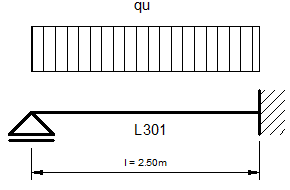
\includegraphics[scale = 0.8]{chapters/chapter_1/images/l301.png}
\end{center}
\end{figure}
\begin{align*}
& D = 588 \frac{Kg}{m^2}\\
& Dtanques = 1200 \frac{Kg}{m^2}\\
& L = 300 \frac{Kg}{m^2} \rightarrow \text{Según CIRSOC 101-05 - Capítulo 4}\\
& q_u = 1.2 \cdot D + 1.6 \cdot L = 1.2 \cdot 588 \frac{Kg}{m^2} + 1.6 \cdot 300 \frac{Kg}{m^2} = 1185.6 \frac{Kg}{m^2} \Rightarrow 1.18 \frac{t}{m^2}\\
& q_u = 1.4 \cdot (D + Dtanques) = 1.4 \cdot (588 \frac{Kg}{m^2} + 1200 \frac{Kg}{m^2})= 2503.2 \frac{Kg}{m^2} \Rightarrow \framebox{$2.50 \frac{t}{m^2}$}\\
& Mu_{empotrado} = \frac{q_u \cdot l^2}{8} = \frac{2.50 \frac{t}{m^2} \cdot (2.50m)^2}{8} = \framebox{$1.95 \frac{t \cdot m}{m}$}\\
& Mu_{tramo} = \frac{9}{128} \cdot q \cdot l^2 = \frac{9}{128} \cdot 2.50 \frac{t}{m^2} \cdot (2.50m)^2 = \framebox{$1.09 \frac{t \cdot m}{m}$}
\end{align*}
\newpage
\item Losa L302: Azotea accesible privadamente

\begin{figure}[H]
\begin{center}
     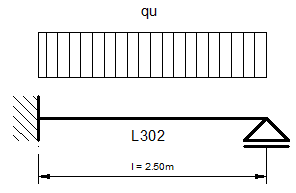
\includegraphics[scale = 0.8]{chapters/chapter_1/images/l302.png}
\end{center}
\end{figure}
\begin{align*}
& D = 588 \frac{Kg}{m^2}\\
& L = 300 \frac{Kg}{m^2} \rightarrow \text{Según CIRSOC 101-05 - Capítulo 4}\\
& q_u = 1.2 \cdot D + 1.6 \cdot L = 1.2 \cdot 588 \frac{Kg}{m^2} + 1.6 \cdot 300 \frac{Kg}{m^2} = 1185.6 \frac{Kg}{m^2} \Rightarrow \framebox{$1.18 \frac{t}{m^2}$}\\
& q_u = 1.4 \cdot D = 1.4 \cdot 588 \frac{Kg}{m^2} = 823.2 \frac{Kg}{m^2} \Rightarrow 0.82 \frac{t}{m^2}\\
& Mu_{empotrado} = \frac{q_u \cdot l^2}{8} = \frac{1.18 \frac{t}{m^2} \cdot (2.50m)^2}{8} = \framebox{$0.92 \frac{t \cdot m}{m}$}\\
& Mu_{tramo} = \frac{9}{128} \cdot q \cdot l^2 = \frac{9}{128} \cdot 1.18 \frac{t}{m^2} \cdot (2.50m)^2 = \framebox{$0.51 \frac{t \cdot m}{m}$}
\end{align*}
\newpage
\item Losa L304: Azotea accesible privadamente

\begin{figure}[H]
\begin{center}
     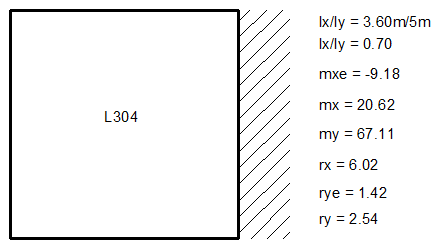
\includegraphics[scale = 0.8]{chapters/chapter_1/images/l304.png}
\end{center}
\end{figure}
\begin{align*}
& D = 588 \frac{Kg}{m^2}\\
& L = 300 \frac{Kg}{m^2} \rightarrow \text{Según CIRSOC 101-05 - Capítulo 4}\\
& q_u = 1.2 \cdot D + 1.6 \cdot L = 1.2 \cdot 588 \frac{Kg}{m^2} + 1.6 \cdot 300 \frac{Kg}{m^2} = 1185.6 \frac{Kg}{m^2} \Rightarrow \framebox{$1.18 \frac{t}{m^2}$}\\
& q_u = 1.4 \cdot D = 1.4 \cdot 588 \frac{Kg}{m^2} = 823.2 \frac{Kg}{m^2} \Rightarrow 0.82 \frac{t}{m^2}\\
& Mu_{xe} = \frac{q_u \cdot (l_{menor})^2}{m_{xe}} = \frac{1.18 \frac{t}{m^2} \cdot (3.60m)^2}{9.18} \framebox{$1.66 \frac{t \cdot m}{m}$}\\
& Mu_x = \frac{q_u \cdot (l_{menor})^2}{m_{x}} = \frac{1.18 \frac{t}{m^2} \cdot (3.60m)^2}{20.62} \framebox{$0.74 \frac{t \cdot m}{m}$}\\
& Mu_y = \frac{q_u \cdot (l_{menor})^2}{m_{y}} = \frac{1.18 \frac{t}{m^2} \cdot (3.60m)^2}{67.11} \framebox{$0.22 \frac{t \cdot m}{m}$}
\end{align*}
\newpage
\item Losa L305: Azotea accesible privadamente

\begin{figure}[H]
\begin{center}
     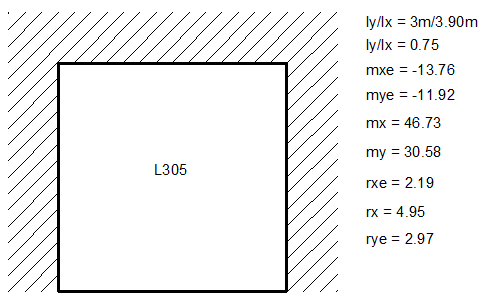
\includegraphics[scale = 0.8]{chapters/chapter_1/images/l305.png}
\end{center}
\end{figure}
\begin{align*}
& D = 588 \frac{Kg}{m^2}\\
& L = 300 \frac{Kg}{m^2} \rightarrow \text{Según CIRSOC 101-05 - Capítulo 4}\\
& q_u = 1.2 \cdot D + 1.6 \cdot L = 1.2 \cdot 588 \frac{Kg}{m^2} + 1.6 \cdot 300 \frac{Kg}{m^2} = 1185.6 \frac{Kg}{m^2} \Rightarrow \framebox{$1.18 \frac{t}{m^2}$}\\
& q_u = 1.4 \cdot D = 1.4 \cdot 588 \frac{Kg}{m^2} = 823.2 \frac{Kg}{m^2} \Rightarrow 0.82 \frac{t}{m^2}\\
& Mu_{xe} = \frac{q_u \cdot (l_{menor})^2}{m_{xe}} = \frac{1.18 \frac{t}{m^2} \cdot (3m)^2}{13.76} \framebox{$0.77 \frac{t \cdot m}{m}$}\\
& Mu_{ye} = \frac{q_u \cdot (l_{menor})^2}{m_{ye}} = \frac{1.18 \frac{t}{m^2} \cdot (3m)^2}{11.92} \framebox{$0.89 \frac{t \cdot m}{m}$}\\
& Mu_x = \frac{q_u \cdot (l_{menor})^2}{m_{x}} = \frac{1.18 \frac{t}{m^2} \cdot (3m)^2}{46.73} \framebox{$0.22 \frac{t \cdot m}{m}$}\\
& Mu_y = \frac{q_u \cdot (l_{menor})^2}{m_{y}} = \frac{1.18 \frac{t}{m^2} \cdot (3m)^2}{30.58} \framebox{$0.34 \frac{t \cdot m}{m}$}
\end{align*}
\newpage
\item Losa L306: Azotea accesible privadamente


\begin{figure}[H]
\begin{center}
     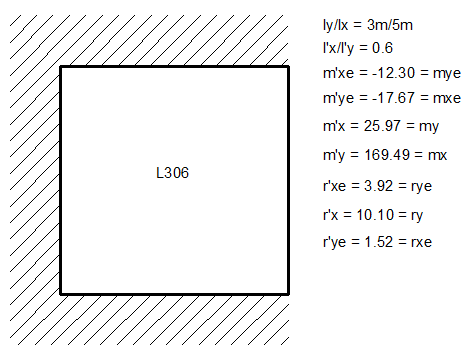
\includegraphics[scale = 0.8]{chapters/chapter_1/images/l306.png}
\end{center}
\end{figure}
\begin{align*}
& D = 588 \frac{Kg}{m^2}\\
& L = 300 \frac{Kg}{m^2} \rightarrow \text{Según CIRSOC 101-05 - Capítulo 4}\\
& q_u = 1.2 \cdot D + 1.6 \cdot L = 1.2 \cdot 588 \frac{Kg}{m^2} + 1.6 \cdot 300 \frac{Kg}{m^2} = 1185.6 \frac{Kg}{m^2} \Rightarrow \framebox{$1.18 \frac{t}{m^2}$}\\
& q_u = 1.4 \cdot D = 1.4 \cdot 588 \frac{Kg}{m^2} = 823.2 \frac{Kg}{m^2} \Rightarrow 0.82 \frac{t}{m^2}\\
& Mu_{xe} = \frac{q_u \cdot (l_{menor})^2}{m_{xe}} = \frac{1.18 \frac{t}{m^2} \cdot (3m)^2}{17.67} \framebox{$0.60 \frac{t \cdot m}{m}$}\\
& Mu_{ye} = \frac{q_u \cdot (l_{menor})^2}{m_{ye}} = \frac{1.18 \frac{t}{m^2} \cdot (3m)^2}{12.30} \framebox{$0.86 \frac{t \cdot m}{m}$}\\
& Mu_x = \frac{q_u \cdot (l_{menor})^2}{m_{x}} = \frac{1.18 \frac{t}{m^2} \cdot (3m)^2}{169.49} \framebox{$0.062 \frac{t \cdot m}{m}$}\\
& Mu_y = \frac{q_u \cdot (l_{menor})^2}{m_{y}} = \frac{1.18 \frac{t}{m^2} \cdot (3m)^2}{25.97} \framebox{$0.40 \frac{t \cdot m}{m}$}
\end{align*}
\newpage
\item Losa L307: Azotea accesible privadamente

\begin{figure}[H]
\begin{center}
     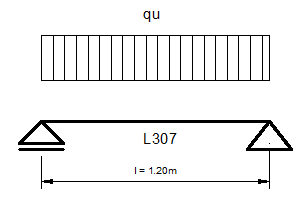
\includegraphics[scale = 0.8]{chapters/chapter_1/images/l307.png}
\end{center}
\end{figure}
\begin{align*}
& D = 588 \frac{Kg}{m^2}\\
& L = 300 \frac{Kg}{m^2} \rightarrow \text{Según CIRSOC 101-05 - Capítulo 4}\\
& q_u = 1.2 \cdot D + 1.6 \cdot L = 1.2 \cdot 588 \frac{Kg}{m^2} + 1.6 \cdot 300 \frac{Kg}{m^2} = 1185.6 \frac{Kg}{m^2} \Rightarrow \framebox{$1.18 \frac{t}{m^2}$}\\
& q_u = 1.4 \cdot D = 1.4 \cdot 588 \frac{Kg}{m^2} = 823.2 \frac{Kg}{m^2} \Rightarrow 0.82 \frac{t}{m^2}\\
& Mu_{tramo} = \frac{q_u \cdot l^2}{8} = \frac{1.18 \frac{t}{m^2} \cdot (1.20m)^2}{8} = \framebox{$0.21 \frac{t \cdot m}{m}$}
\end{align*}
\newpage
\item Losa L308: Azotea accesible privadamente

\begin{figure}[H]
\begin{center}
     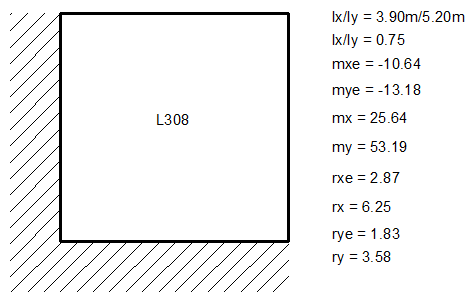
\includegraphics[scale = 0.8]{chapters/chapter_1/images/l308.png}
\end{center}
\end{figure}
\begin{align*}
& D = 588 \frac{Kg}{m^2}\\
& L = 300 \frac{Kg}{m^2} \rightarrow \text{Según CIRSOC 101-05 - Capítulo 4}\\
& q_u = 1.2 \cdot D + 1.6 \cdot L = 1.2 \cdot 588 \frac{Kg}{m^2} + 1.6 \cdot 300 \frac{Kg}{m^2} = 1185.6 \frac{Kg}{m^2} \Rightarrow \framebox{$1.18 \frac{t}{m^2}$}\\
& q_u = 1.4 \cdot D = 1.4 \cdot 588 \frac{Kg}{m^2} = 823.2 \frac{Kg}{m^2} \Rightarrow 0.82 \frac{t}{m^2}\\
& Mu_{xe} = \frac{q_u \cdot (l_{menor})^2}{m_{xe}} = \frac{1.18 \frac{t}{m^2} \cdot (3.90m)^2}{10.64} \framebox{$1.68 \frac{t \cdot m}{m}$}\\
& Mu_{ye} = \frac{q_u \cdot (l_{menor})^2}{m_{ye}} = \frac{1.18 \frac{t}{m^2} \cdot (3.90m)^2}{13.18} \framebox{$1.36 \frac{t \cdot m}{m}$}\\
& Mu_x = \frac{q_u \cdot (l_{menor})^2}{m_{x}} = \frac{1.18 \frac{t}{m^2} \cdot (3.90m)^2}{25.64} \framebox{$0.69 \frac{t \cdot m}{m}$}\\
& Mu_y = \frac{q_u \cdot (l_{menor})^2}{m_{y}} = \frac{1.18 \frac{t}{m^2} \cdot (3.90m)^2}{53.19} \framebox{$0.33 \frac{t \cdot m}{m}$}
\end{align*}
\newpage
\item Losa L309: Azotea accesible privadamente

\begin{figure}[H]
\begin{center}
     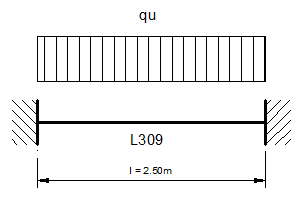
\includegraphics[scale = 0.8]{chapters/chapter_1/images/l309.png}
\end{center}
\end{figure}
\begin{align*}
& D = 588 \frac{Kg}{m^2}\\
& L = 300 \frac{Kg}{m^2} \rightarrow \text{Según CIRSOC 101-05 - Capítulo 4}\\
& q_u = 1.2 \cdot D + 1.6 \cdot L = 1.2 \cdot 588 \frac{Kg}{m^2} + 1.6 \cdot 300 \frac{Kg}{m^2} = 1185.6 \frac{Kg}{m^2} \Rightarrow \framebox{$1.18 \frac{t}{m^2}$}\\
& q_u = 1.4 \cdot D = 1.4 \cdot 588 \frac{Kg}{m^2} = 823.2 \frac{Kg}{m^2} \Rightarrow 0.82 \frac{t}{m^2}\\
& Mu_{empotrado} = \frac{q_u \cdot l^2}{12} = \frac{1.18 \frac{t}{m^2} \cdot (2.50m)^2}{12} = \framebox{$0.61 \frac{t \cdot m}{m}$}\\
& Mu_{tramo} = \frac{q_u \cdot l^2}{24} = \frac{1.18 \frac{t}{m^2} \cdot (2.50m)^2}{24} = \framebox{$0.30 \frac{t \cdot m}{m}$}
\end{align*}
\newpage
\item Losa L310: Azotea accesible privadamente

\begin{figure}[H]
\begin{center}
     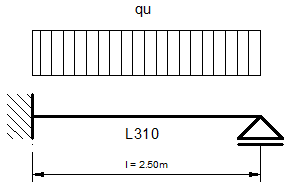
\includegraphics[scale = 0.8]{chapters/chapter_1/images/l310.png}
\end{center}
\end{figure}
\begin{align*}
& D = 588 \frac{Kg}{m^2}\\
& L = 300 \frac{Kg}{m^2} \rightarrow \text{Según CIRSOC 101-05 - Capítulo 4}\\
& q_u = 1.2 \cdot D + 1.6 \cdot L = 1.2 \cdot 588 \frac{Kg}{m^2} + 1.6 \cdot 300 \frac{Kg}{m^2} = 1185.6 \frac{Kg}{m^2} \Rightarrow \framebox{$1.18 \frac{t}{m^2}$}\\
& q_u = 1.4 \cdot D = 1.4 \cdot 588 \frac{Kg}{m^2} = 823.2 \frac{Kg}{m^2} \Rightarrow 0.82 \frac{t}{m^2}\\
& Mu_{empotrado} = \frac{q_u \cdot l^2}{8} = \frac{1.18 \frac{t}{m^2} \cdot (2.50m)^2}{8} = \framebox{$0.92 \frac{t \cdot m}{m}$}\\
& Mu_{tramo} = \frac{9}{128} \cdot q \cdot l^2 = \frac{9}{128} \cdot 1.18 \frac{t}{m^2} \cdot (2.50m)^2 = \framebox{$0.51 \frac{t \cdot m}{m}$}
\end{align*}
\newpage
\item Losa L311: Azotea accesible privadamente

\begin{figure}[H]
\begin{center}
     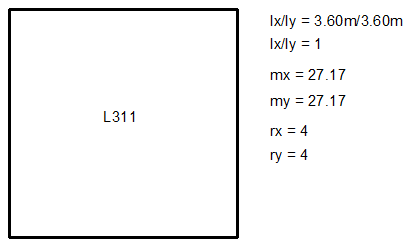
\includegraphics[scale = 0.8]{chapters/chapter_1/images/l311.png}
\end{center}
\end{figure}
\begin{align*}
& D = 588 \frac{Kg}{m^2}\\
& L = 300 \frac{Kg}{m^2} \rightarrow \text{Según CIRSOC 101-05 - Capítulo 4}\\
& q_u = 1.2 \cdot D + 1.6 \cdot L = 1.2 \cdot 588 \frac{Kg}{m^2} + 1.6 \cdot 300 \frac{Kg}{m^2} = 1185.6 \frac{Kg}{m^2} \Rightarrow \framebox{$1.18 \frac{t}{m^2}$}\\
& q_u = 1.4 \cdot D = 1.4 \cdot 588 \frac{Kg}{m^2} = 823.2 \frac{Kg}{m^2} \Rightarrow 0.82 \frac{t}{m^2}\\
& Mu_x = Mu_y = \frac{q_u \cdot (l_{menor})^2}{m_{x}} = \frac{1.18 \frac{t}{m^2} \cdot (3.60m)^2}{27.17} \framebox{$0.56 \frac{t \cdot m}{m}$}\\
\end{align*}

\end{itemize}
\newpage
\item \underline{Compatibilización de Momentos - Nivel 3}\\

\begin{itemize}
\item Losas L301 y L302
\begin{align*}
& (1.95-0.92) < 0.40 \cdot \frac{(1.95+0.92)}{2}\\
& 1.03 < 0.57 \Rightarrow \quad \text{No Verifica}\\
& \text{Adopto} \quad \framebox{1.43} \quad \text{en el apoyo}\\
& 1.09 + (1.95-1.43) = 1.61\\
& \text{Adopto} \quad \framebox{1.61} \quad \text{en el tramo}\\
\end{align*}

\item Losas L304 y L308
\begin{align*}
& (1.68-1.66) < 0.40 \cdot \frac{(1.68+1.66)}{2}\\
& 0.02 < 0.66 \Rightarrow \quad \text{Verifica}\\
& \text{Adopto} \quad \framebox{1.67} \quad \text{en el apoyo}\\
& 0.69 + (1.68-1.67) = 0.70\\
& \text{Adopto} \quad \framebox{0.70} \quad \text{en el tramo}\\
\end{align*}

\item Losas L305 y L308
\begin{align*}
& (1.36-0.89) < 0.40 \cdot \frac{(1.36+0.89)}{2}\\
& 0.47 < 0.45 \Rightarrow \quad \text{No Verifica}\\
& \text{Adopto} \quad \framebox{1.12} \quad \text{en el apoyo}\\
& 0.33 + (1.36-1.12) = 0.57\\
& \text{Adopto} \quad \framebox{0.57} \quad \text{en el tramo}\\
\end{align*}

\item Losas L305 y L306
\begin{align*}
& (0.77-0.60) < 0.40 \cdot \frac{(0.77+0.60)}{2}\\
& 0.17 < 0.27 \Rightarrow \quad \text{Verifica}\\
& \text{Adopto} \quad \framebox{0.68} \quad \text{en el apoyo}\\
& 0.22 + (0.77-0.68) = 0.31\\
& \text{Adopto} \quad \framebox{0.31} \quad \text{en el tramo}\\
\end{align*}

\item Losas L309 y L310
\begin{align*}
& (0.92-0.61) < 0.40 \cdot \frac{(0.92+0.61)}{2}\\
& 0.31 < 0.30 \Rightarrow \quad \text{No Verifica}\\
& \text{Adopto} \quad \framebox{0.76} \quad \text{en el apoyo}\\
& 0.51 + (0.92-0.76) = 0.67\\
& \text{Adopto} \quad \framebox{0.67} \quad \text{en el tramo}\\
\end{align*}
\end{itemize}

La diferencia entre los momentos superan el 40\% del promedio de los mismos, adoptamos de todas formas el valor promedio dado que esta diferencia es mínima.
\newpage
\item \underline{Cálculo de Armaduras}\\
Se calcula la armadura para los momentos máximos obtenidos.
\begin{itemize}
\item Armadura Superior

\begin{align*}
& M_u = 1.67 \frac{t \cdot m}{m} \\
& M_n = \frac{M_u}{\phi} = \frac{1.67 \frac{t \cdot m}{m}}{0.9} = 1.85 \frac{t \cdot m}{m} \Rightarrow 0.0185 \frac{MN \cdot m}{m} \\
& d = h -db - Cc - \frac{db}{2} = 14cm - 0.8cm - 2cm - \frac{0.8cm}{2}= 10.8cm \\
& Kd = \frac{d}{\sqrt{\frac{M_n}{b}}} = \frac{0.108m}{\sqrt[]{\frac{0.0185 \frac{MN \cdot m}{m}}{1m}}} = 0.794 \Rightarrow Ke = 24.766 \\
& A_s = Ke \cdot \frac{M_n}{d} = 24.766 \cdot \frac{0.0185 \frac{MN \cdot m}{m}}{0.108m} = \framebox{$4.24 \frac{cm^2}{m}$}\\
& As_{min} = 0.0018 \cdot b \cdot h = 0.0018 \cdot 100cm \cdot 14cm = 2.52 \frac{cm^2}{m}
\end{align*}
La armadura mínima se cubre con $\phi$ 8 cada 20cm $\rightarrow \framebox{$2.51 \frac{cm^2}{m}$}$ \\
\\
Se adopta A° superior $\phi$ 8 cada 10cm $\rightarrow \framebox{$5.03 \frac{cm^2}{m}$}$ \\

\underline{Verificación de separaciones}\\

\[ s = 10cm \leq \left\{ \begin{array}{ll}
         2.5 \cdot h = 2.5 \cdot 14cm = 35cm \quad \surd & \\
         25 \cdot db = 25 \cdot 0.8cm = 20cm \quad \surd &\\
         30cm \quad \surd & \end{array} \right. \] 
         
\[ s = 10cm \geq \left\{ \begin{array}{ll}
         db = 0.8cm \quad \surd & \\
         \geq 2.5cm \quad \surd &\\
         \geq \frac{4}{3} \cdot \text{Tamaño máximo del agregado} & \end{array} \right. \] 

\item Armadura Inferior

\begin{align*}
& M_u = 1.61 \frac{t \cdot m}{m} \\
& M_n = \frac{M_u}{\phi} = \frac{1.61 \frac{t \cdot m}{m}}{0.9} = 1.78 \frac{t \cdot m}{m} \Rightarrow 0.0178 \frac{MN \cdot m}{m} \\
& d = h -db - Cc - \frac{db}{2} = 14cm - 0.8cm - 2cm - \frac{0.8cm}{2}= 10.8cm \\
& Kd = \frac{d}{\sqrt{\frac{M_n}{b}}} = \frac{0.108m}{\sqrt[]{\frac{0.0178 \frac{MN \cdot m}{m}}{1m}}} = 0.809 \Rightarrow Ke = 24.734 \\
& A_s = Ke \cdot \frac{M_n}{d} = 24.734 \cdot \frac{0.0178 \frac{MN \cdot m}{m}}{0.108m} = \framebox{$4.07 \frac{cm^2}{m}$}\\
& As_{min} = 0.0018 \cdot b \cdot h = 0.0018 \cdot 100cm \cdot 14cm = 2.52 \frac{cm^2}{m}
\end{align*}
La armadura mínima se cubre con $\phi$ 8 cada 20cm $\rightarrow \framebox{$2.51 \frac{cm^2}{m}$}$ \\
\\
Se adopta A° inferior $\phi$ 8 cada 12cm $\rightarrow \framebox{$4.19 \frac{cm^2}{m}$}$ \\

\underline{Verificación de separaciones}\\

\[ s = 12cm \leq \left\{ \begin{array}{ll}
         2.5 \cdot h = 2.5 \cdot 14cm = 35cm \quad \surd & \\
         25 \cdot db = 25 \cdot 0.8cm = 20cm \quad \surd &\\
         30cm \quad \surd & \end{array} \right. \] 
         
\[ s = 12cm \geq \left\{ \begin{array}{ll}
         db = 0.8cm \quad \surd & \\
         \geq 2.5cm \quad \surd &\\
         \geq \frac{4}{3} \cdot \text{Tamaño máximo del agregado} & \end{array} \right. \] 

A continuación calculamos la armadura para una nueva pareja de momentos con el fin de optimizar el armado.\\
\item Armadura Superior

\begin{align*}
& M_u = 1.43 \frac{t \cdot m}{m} \\
& M_n = \frac{M_u}{\phi} = \frac{1.43 \frac{t \cdot m}{m}}{0.9} = 1.58 \frac{t \cdot m}{m} \Rightarrow 0.0158 \frac{MN \cdot m}{m} \\
& d = h -db - Cc - \frac{db}{2} = 14cm - 0.8cm - 2cm - \frac{0.8cm}{2}= 10.8cm \\
& Kd = \frac{d}{\sqrt{\frac{M_n}{b}}} = \frac{0.108m}{\sqrt[]{\frac{0.0158 \frac{MN \cdot m}{m}}{1m}}} = 0.859 \Rightarrow Ke = 24.622 \\
& A_s = Ke \cdot \frac{M_n}{d} = 24.622 \cdot \frac{0.0158 \frac{MN \cdot m}{m}}{0.108m} = \framebox{$3.60 \frac{cm^2}{m}$}\\
& As_{min} = 0.0018 \cdot b \cdot h = 0.0018 \cdot 100cm \cdot 14cm = 2.52 \frac{cm^2}{m}
\end{align*}
La armadura mínima se cubre con $\phi$ 8 cada 20cm $\rightarrow \framebox{$2.51 \frac{cm^2}{m}$}$ \\
\\
Se adopta A° superior $\phi$ 8 cada 12cm $\rightarrow \framebox{$4.19 \frac{cm^2}{m}$}$ \\

\underline{Verificación de separaciones}\\

\[ s = 12cm \leq \left\{ \begin{array}{ll}
         2.5 \cdot h = 2.5 \cdot 14cm = 35cm \quad \surd & \\
         25 \cdot db = 25 \cdot 0.8cm = 20cm \quad \surd &\\
         30cm \quad \surd & \end{array} \right. \] 
         
\[ s = 12cm \geq \left\{ \begin{array}{ll}
         db = 0.8cm \quad \surd & \\
         \geq 2.5cm \quad \surd &\\
         \geq \frac{4}{3} \cdot \text{Tamaño máximo del agregado} & \end{array} \right. \] 

\item Armadura Inferior

\begin{align*}
& M_u = 0.93 \frac{t \cdot m}{m} \\
& M_n = \frac{M_u}{\phi} = \frac{0.93 \frac{t \cdot m}{m}}{0.9} = 1.03 \frac{t \cdot m}{m} \Rightarrow 0.010 \frac{MN \cdot m}{m} \\
& d = h -db - Cc - \frac{db}{2} = 14cm - 0.8cm - 2cm - \frac{0.8cm}{2}= 10.8cm \\
& Kd = \frac{d}{\sqrt{\frac{M_n}{b}}} = \frac{0.108m}{\sqrt[]{\frac{0.010 \frac{MN \cdot m}{m}}{1m}}} = 1.06 \Rightarrow Ke = 24.332 \\
& A_s = Ke \cdot \frac{M_n}{d} = 24.332 \cdot \frac{0.010 \frac{MN \cdot m}{m}}{0.108m} = \framebox{$2.25 \frac{cm^2}{m}$}\\
& As_{min} = 0.0018 \cdot b \cdot h = 0.0018 \cdot 100cm \cdot 14cm = 2.52 \frac{cm^2}{m}
\end{align*}
La armadura mínima se cubre con $\phi$ 8 cada 20cm $\rightarrow \framebox{$2.51 \frac{cm^2}{m}$}$ \\
\\
Se adopta A° inferior $\phi$ 8 cada 20cm $\rightarrow \framebox{$2.51 \frac{cm^2}{m}$}$ \\

\underline{Verificación de separaciones}\\

\[ s = 20cm \leq \left\{ \begin{array}{ll}
         2.5 \cdot h = 2.5 \cdot 14cm = 35cm \quad \surd & \\
         25 \cdot db = 25 \cdot 0.8cm = 20cm \quad \surd &\\
         30cm \quad \surd & \end{array} \right. \] 
         
\[ s = 20cm \geq \left\{ \begin{array}{ll}
         db = 0.8cm \quad \surd & \\
         \geq 2.5cm \quad \surd &\\
         \geq \frac{4}{3} \cdot \text{Tamaño máximo del agregado} & \end{array} \right. \] 

\end{itemize}
\end{enumerate}
